% $Header: svn+ssh://andre@crapman/home/junda/repos/andre/school/trunk/m/Chapter/stat/probability/prob.main.tex 303 2023-03-09 16:02:30Z andre $

\newif\ifteacher
% \teachertrue
\teacherfalse

%%aspectratio=1610;169;149;54;43(default);32
% % \documentclass[fleqn,11pt,trans,aspectratio=169]{beamer}
% % \documentclass[fleqn,11pt,article,aspectratio=43]{beamer}
% % \documentclass[fleqn,11pt,handout,aspectratio=43]{beamer}
% \documentclass[fleqn,11pt,trans,aspectratio=43,hyperref={colorlinks = true,linkcolor = blue}]{beamer}
\ifteacher\documentclass[fleqn,11pt,beamer,aspectratio=43,hyperref={colorlinks = true,linkcolor = blue,urlcolor=red!30!black}]{beamer}
\else \documentclass[fleqn,11pt,handout,hyperref={colorlinks = true,linkcolor = blue,urlcolor=red!30!black}]{beamer}
\fi
\def\adVers{202509.v.0.01}


\newif\iflong

% This file is a solution template for:

% - Talk at a conference/colloquium.
% - Talk length is about 20min.
% - Style is ornate.



% Copyright 2004 by Till Tantau <tantau@users.sourceforge.net>.
%
% In principle, this file can be redistributed and/or modified under
% the terms of the GNU Public License, version 2.
%
% However, this file is supposed to be a template to be modified
% for your own needs. For this reason, if you use this file as a
% template and not specifically distribute it as part of a another
% package/program, I grant the extra permission to freely copy and
% modify this file as you see fit and even to delete this copyright
% notice.


\mode<presentation>
{
%  \usetheme{Warsaw}
%  \usetheme{Antibes}
% \usetheme[secheader]{Madrid}
\usetheme[]{Madrid}
% AnnArbor
% Antibes
% Bergen
% Berkeley
% Berlin
% \usetheme[Boadilla}
% boxes
% CambridgeUS
% Copenhagen
% Darmstadt
% default
% Dresden
% Frankfurt
% Goettingen
% Hannover
% Ilmenau
% JuanLesPins
% Luebeck
% Madrid
% Malmoe
% Marburg
% Montpellier
% PaloAlto
% Pittsburgh
% Rochester
% Singapore
% Szeged
% Warsaw

  \setbeamercovered{transparent}
  \setbeamertemplate{blocks}[default]
  % or whatever (possibly just delete it)
  \usecolortheme{seahorse}%%
}

\mode<handout>{
  \usetheme{default}
  \usecolortheme{dove}
  %   \setbeamercolor{background canvas}{bg=white}%black!5}
}
  
\title[Physik: klassische Mechanik] % (optional, use only with long paper titles)
{Physik: klassische Mechanik}

% \subtitle
% {Include Only If Paper Has a Subtitle}

% \author[Dostal] % (optional, use only with lots of authors)
% {Andr\'e Dostal}
% - Give the names in the same order as the appear in the paper.
% - Use the \inst{?} command only if the authors have different
%   affiliation.

\institute[\adVers \copyright ad7@gmx.at] % (optional, but mostly needed)
% \institute[Universities of Somewhere and Elsewhere] % (optional, but mostly needed)
% {
%   \inst{1}%
%   Department of Computer Science\\
%   University of Somewhere
%   \and
%   \inst{2}%
%   Department of Theoretical Philosophy\\
%   University of Elsewhere}
% - Use the \inst command only if there are several affiliations.
% - Keep it simple, no one is interested in your street address.

\date[2025/26] % (optional, should be abbreviation of conference name)
{2025/26}
% - Either use conference name or its abbreviation.
% - Not really informative to the audience, more for people (including
%   yourself) who are reading the slides online

\subject{Physik: klassische Mechanik}
% This is only inserted into the PDF information catalog. Can be left
% out.

\usepackage[ngerman,english]{babel}
% or whatever
\usepackage[
    style=alphabetic,
%     style=authoryear,
    % refsegment=chapter,
    refsegment=section,
%     refsection=chapter,
    backend=biber,
    hyperref=true
    ]{biblatex}
% \defbibheading{subbibliography}{\vspace{-0.5\baselineskip}}
% \defbibheading{onlinesources}{\section*{Online Sources}}
% \defbibheading{printedsources}{\section*{Printed Sources}}
\defbibheading{subbib}{\section*{References}}
%%linebreak in urls
\setcounter{biburlnumpenalty}{9000}
\setcounter{biburlucpenalty}{9000}
\setcounter{biburllcpenalty}{9000}

\addbibresource{./bibbook/ph.bib}
\renewcommand*{\citesetup}{%
  \scriptsize
  \biburlsetup
  \frenchspacing}


% \usepackage[latin1]{inputenc}
\usepackage[utf8]{inputenc}
% or whatever

% \usepackage{times}
\usepackage[T1]{fontenc}
% \usepackage{times}
\usepackage{ebgaramond-maths}
\usepackage{ebgaramond}

% \usepackage{arevmath}
\usefonttheme{professionalfonts}
\usefonttheme[]{serif}
\usefonttheme[]{structuresmallcapsserif}

% \fontsize{6}{3}{
%     }
% \makeatletter
% \DeclareMathSizes{\@xpt}{7}{6}{5}
% \DeclareMathSizes{\@xipt}{9}{6}{5}
% % \DeclareMathSizes{\@xiipt}{9}{7}{6}
% % \DeclareMathSizes{\@xiipt}{11}{7}{6}
% \DeclareMathSizes{\@xivpt}{\@xivpt}{\@xpt}{7}
% \DeclareMathSizes{\@xviipt}{\@xviipt}{\@xiipt}{\@xpt}
% \DeclareMathSizes{\@xxpt}{\@xxpt}{\@xivpt}{\@xiipt}
% \DeclareMathSizes{\@xxvpt}{\@xxvpt}{\@xxpt}{\@xviipt}
% \makeatother


% Or whatever. Note that the encoding and the font should match. If T1
% does not look nice, try deleting the line with the fontenc.
%%\usepackage[dvipdfm]{graphicx}
\usepackage[]{graphicx}
\usepackage{units}
% \usepackage{siunitx}
%
\usepackage{pgf,tikz}
\usetikzlibrary{arrows}
% \usetikzlibrary{automata}
\usetikzlibrary{arrows.meta}
% \usetikzlibrary{intersections}
\usetikzlibrary{calc}
\usetikzlibrary{chains}
% \usetikzlibrary{math}
\usetikzlibrary{patterns}
% \usetikzlibrary{trees}
% \usetikzlibrary{plothandlers}
% \graphicspath{{./plots/}}
% \usetikzlibrary{graphs}
\usetikzlibrary {positioning}
\usepackage[]{tikzpeople}
\usetikzlibrary{shapes.callouts}
\usetikzlibrary{shadows}
\usetikzlibrary{external}

\usepackage{pgfplots}
\pgfplotsset{compat=1.16}
\usepgfplotslibrary{fillbetween}

\pgfdeclareverticalshading{rainbow}{100bp}
 {color(0bp)=(red); color(25bp)=(red); color(35bp)=(yellow);
  color(45bp)=(green); color(55bp)=(cyan); color(65bp)=(blue);
  color(75bp)=(violet); color(100bp)=(violet)}

\usepackage{pgfpages}
% \pgfpagesuselayout{resize to}[a4paper,border shrink=5mm,landscape]
% \pgfpagesuselayout{4 on 1}[a4paper,border shrink=5mm,landscape]
\mode<handout>{
  \pgfpagesuselayout{2 on 1}[a4paper,border shrink=2mm]
%   \pgfpagesuselayout{4 on 1}[a4paper,border shrink=4mm,landscape]
}

\usepackage{multimedia}

% \usepackage[urlcolor=red]{hyperref}%%loaded by beamer by default
% \usepackage{url}
\usepackage{amsmath}
\usepackage{wasysym}
\let\SAVEDRightarrow=\Rightarrow
\usepackage{marvosym}
\let\Rightarrow=\SAVEDRightarrow
% \usepackage{ifsym} %%strichliste
\usepackage{eurosym}
\usepackage{color}
% \usepackage{fourier}
\usepackage{cancel}
% \usepackage{enumitem} %%labelind
\usepackage{tabularray}%%https://at.ctan.niranjan.co/macros/latex/contrib/tabularray/tabularray.pdf
% \usepackage{booktabs}
% \usepackage{array}
\usepackage{tikzlings-bears}
% \usepackage{tikzlings}

% \usepackage{mhchem}%%

%%==============================================================================
%% radiant in school book style
\newcommand{\tarc}{\mbox{$\frown$}}
\newcommand{\arc}[2][-0.7em]{{#2}{\kern #1{\raisebox{1.5ex}{\tarc}}}}
%%==============================================================================

%%==============================================================================
%% d in integral should be upright
\newcommand*\diff{\mathop{}\!\mathrm{d}}
%%==============================================================================
\newcommand{\adborn}{{\usefont{T1}{cmr}{m}{n}\textborn}}
\newcommand{\addied}{{\usefont{T1}{cmr}{m}{n}\textdied}}



% If you have a file called "university-logo-filename.xxx", where xxx
% is a graphic format that can be processed by latex or pdflatex,
% resp., then you can add a logo as follows:

% \pgfdeclareimage[height=0.5cm]{university-logo}{university-logo-filename}
% \logo{\pgfuseimage{university-logo}}



% Delete this, if you do not want the table of contents to pop up at
% the beginning of each subsection:
% \AtBeginSubsection[]
% {
%   \begin{frame}<beamer>
%     \frametitle{Outline}
%     \tableofcontents[currentsection,currentsubsection]
%   \end{frame}
% }


% If you wish to uncover everything in a step-wise fashion, uncomment
% the following command:

%\beamerdefaultoverlayspecification{<+->}

% \pgfplotsset{ % Define a common style, so we don't repeat ourselves
%     MaoYiyi/.style={
% %         width=0.6\textwidth, % Overall width of the plot
%         axis equal image, % Unit vectors for both axes have the same length
%         view={0}{90}, % We need to use "3D" plots, but we set the view so we look at them from straight up
% %         xmin=0, xmax=1.1, % Axis limits
% %         ymin=0, ymax=1.1,
% %         domain=0:1, y domain=0:1, % Domain over which to evaluate the functions
% %         xtick={0,0.5,1}, ytick={0,0.5,1}, % Tick marks
%         samples=11, % How many arrows?
%         cycle list={    % Plot styles
%                 line width=0.2mm,
%                 gray,
%                 quiver={
%                     u={1}, v={f(x)}, % End points of the arrows
%                     scale arrows=0.075,
% %                     scale arrows=0.075,
% %                     every arrow/.append style={
% %                         {Stealth[length=1mm,round,open]}
% %                         -latex % Arrow tip
% %                     },
%                 }\\
%                 red, samples=31, smooth, thick, no markers, domain=0:1.1\\ % The plot style for the function
%         }
%     }
% }
% \usepackage[os=win]{menukeys}
% \usepackage{libertine}

%%==============================================================================
\newcommand{\keystroke}[1]{{
  \hspace{0.1ex}%%
    \tikz[baseline={([0.15\baselineskip]current bounding box.south)}]%%
%    \tikz[baseline={([yshift=0.15\baselineskip]current bounding box.south)}]%%
%     \tikz[baseline=(ke‌​y.base)]
    \node[%%
      draw,
%       t‌​ext height=1.5ex,text depth=0ex,
      fill=black!10,drop shadow={shadow xshift=0.2ex,shadow yshift=-0.2ex
        ,fill=black,opacity=0.50}
      ,rectangle,rounded corners=2pt,inner sep=2.75pt,line width=0.5pt
      ,font=\footnotesize\sffamily,minimum width=0.3cm
      ] (key) {#1};
   \hspace{0.1ex}%%
}}
%%==============================================================================

%%==============================================================================
%%TR-Tasten
\newcommand{\TRb} [1]{{\tikz [baseline={([yshift=0.15\baselineskip]current bounding box.south)},start chain,node distance=1mm] \foreach \x in {#1} \node [anchor=mid,on chain,draw,rounded corners,font=\footnotesize\sffamily,minimum height=0.30cm,fill=black!10,draw=black     ,rounded corners=2pt,inner sep=2.75pt,line width=0.5pt] {\x}; }}%%inner sep=0.1cm,
\newcommand{\TRr} [1]{{\tikz [baseline={([yshift=0.15\baselineskip]current bounding box.south)},start chain,node distance=1mm] \foreach \x in {#1} \node [anchor=mid,on chain,draw,rounded corners,font=\footnotesize\sffamily,minimum height=0.30cm,fill=red!20,draw=red!80      ,rounded corners=2pt,inner sep=2.75pt,line width=0.5pt] {\x}; }}%%inner sep=0.1cm,
\newcommand{\TRo} [1]{{\tikz [baseline={([yshift=0.15\baselineskip]current bounding box.south)},start chain,node distance=1mm] \foreach \x in {#1} \node [anchor=mid,on chain,draw,rounded corners,font=\footnotesize\sffamily,minimum height=0.30cm,fill=orange!30,draw=orange!80,rounded corners=2pt,inner sep=2.75pt,line width=0.5pt] {\x}; }}%%inner sep=0.1cm,
\newcommand{\TRy} [1]{{\tikz [baseline={([yshift=0.15\baselineskip]current bounding box.south)},start chain,node distance=1mm] \foreach \x in {#1} \node [anchor=mid,on chain,draw,rounded corners,font=\footnotesize\sffamily,minimum height=0.30cm,fill=yellow!30,draw=yellow!90,rounded corners=2pt,inner sep=2.75pt,line width=0.5pt] {\x}; }}%%inner sep=0.1cm,
\newcommand{\TRbl}[1]{{\tikz [baseline={([yshift=0.15\baselineskip]current bounding box.south)},start chain,node distance=1mm] \foreach \x in {#1} \node [anchor=mid,on chain,draw,rounded corners,font=\footnotesize\sffamily,minimum height=0.30cm,fill=blue!30  ,draw=blue!90  ,rounded corners=2pt,inner sep=2.75pt,line width=0.5pt] {\x}; }}%%inner sep=0.1cm,
%%==============================================================================
\newcommand{\keystrokes}[1]{{
  \hspace{0.1ex}%%
    \tikz[baseline={([0.15\baselineskip]current bounding box.south)}
%    \tikz[baseline={([yshift=0.15\baselineskip]current bounding box.south)}

      ,start chain,node distance=1mm]%%
%     \tikz[baseline=(ke‌​y.base)]
%     \foreach \x in {#1}
    \foreach \x [count=\cnt] in {#1}
    \node[%%
      on chain,draw,
%       t‌​ext height=1.5ex,text depth=0ex,
      fill=black!10,drop shadow={shadow xshift=0.2ex,shadow yshift=-0.2ex
        ,fill=black,opacity=0.50}
      ,rectangle,rounded corners=2pt,inner sep=2.75pt,line width=0.5pt
      ,font=\footnotesize\sffamily,minimum width=0.3cm%,shift={{(\xi*0.5-0.5,0)}}
      ] (k-\cnt) {\x};
   \hspace{0.1ex}%%
}}
%%==============================================================================

%%==============================================================================
\newcommand{\adRule}[2]{{%%#deciTics #centiTics
  \makebox[0pt]{|0}%%
  \foreach \n  [count=\ni,evaluate=\n as \npe using \ni+1] in {1,...,#1}{%%
    \parbox{0.1\linewidth}{\,\!}\makebox[0pt]{|\ni}%%
%     \phantom{\ifnum #1<\npe%%
%       \breakforeach%%
%     \fi}%%
  }%%
  \!\!
  \foreach \n  [count=\ni,evaluate=\n as \npe using \ni+1] in {1,...,#2}{%%
    \parbox{0.01\linewidth}{\,\!}\makebox[0pt]{|}%%
%     \phantom{\ifnum #2<\npe%%
%       \breakforeach%%
%     \fi}%%
  }
%     \makebox[0pt]{|}\parbox{0.1\linewidth}{\ }\makebox[0pt]{|}%%
%     \parbox{0.1\linewidth}{\ }\makebox[0pt]{|}%%
%     \parbox{0.01\linewidth}{\ }\makebox[0pt]{|}%%
%     \parbox{0.01\linewidth}{\ }\makebox[0pt]{|}\\%%
}}
%%==============================================================================

%%==============================================================================
\newcommand{\minitab}[2][@{}c@{}]{\begin{tabular}[t]{#1}#2\end{tabular}}
%%==============================================================================
%%==============================================================================
\newcommand{\miniarray}[2][@{}c@{}]{\begin{array}[t]{#1}#2\end{array}}
%%==============================================================================

%%==============================================================================
\newcommand{\adCenter}[1]{\hspace*{\stretch{1}}{#1}\hspace*{\stretch{1}}}
%%==============================================================================

%%==============================================================================
\newcommand{\adBall}[3]{%%color size text
% \tikz{[anchor=base, baseline]\shade[ball color=#1](0,0) circle (#2) node[] {#3}}
% \tikz{[baseline=0pt]\shade[ball color=#1](0,0) circle (#2) node[] {#3}}
% \tikz{[baseline=(x.base)]\shade[ball color=#1](0,0) circle (#2) node[anchor=base,shift={{(0,-0.3ex)}}](x) {#3}}
% \tikz{[baseline=(x.base)]\shade[ball color=#1](0,0) circle (#2) node[anchor=mid](x) {#3}}
% \tikz{[baseline=(x.base)]\shade[ball color=#1](0,0) circle (#2) node[yshift=-0.1\baselineskip,anchor=base](x) {\tiny#3}}
% \tikz{[baseline=(current bounding box.mid)]\shade[ball color=#1](0,0) circle (#2) node[yshift=-0.1\baselineskip,anchor=base](x) {\tiny#3}}
% \tikz{[baseline=(current bounding box.center)]\shade[ball color=#1](0,0) circle (#2) node[yshift=-0.0\baselineskip](x) {#3};}
% \tikz{[baseline=(current bounding box.mid)]\shade[ball color=#1](0,0) circle (#2) node[yshift=-0.0\baselineskip](x) {#3};}
\tikz{[baseline=(current bounding box.base)]\shade[ball color=#1](0,0) circle (#2) node[yshift=-0.0\baselineskip](x) {#3};}
}
%%==============================================================================

%%==============================================================================
\newcommand{\adDiceOne}[1][black]{%%color
\tikz\draw (0,0) node [draw,minimum size=12pt,rounded corners,color=#1]
  {\tikz{ \draw(0,0) node [fill=black,circle,inner sep=0.1mm,outer sep=0pt,minimum size=2pt,color=#1] {}; } };
}
\newcommand{\adDiceTwo}[1][black]{%%color
\tikz\draw (0,0) node [draw,minimum size=12pt,rounded corners,inner sep=0.1mm,outer sep=0pt,color=#1]
  {\tikz{ \foreach \p in {(-3pt,-3pt),(3pt,3pt)}
            \draw \p node [fill=black,circle,inner sep=0.1mm,outer sep=0pt,minimum size=2pt,color=#1] {}; } };
}
\newcommand{\adDiceThree}[1][black]{%%color
\tikz\draw (0,0) node [draw,minimum size=12pt,rounded corners,inner sep=0.1mm,outer sep=0pt,color=#1]
  {\tikz{ \foreach \p in {(0,0),(-3pt,-3pt),(3pt,3pt)}
            \draw \p node [fill=black,circle,inner sep=0.1mm,outer sep=0pt,minimum size=2pt,color=#1] {}; } };
}
\newcommand{\adDiceFour}[1][black]{%%color
\tikz\draw (0,0) node [draw,minimum size=12pt,rounded corners,inner sep=0.1mm,outer sep=0pt,color=#1]
  {\tikz{ \foreach \p in {(-3pt,-3pt),(3pt,3pt),(3pt,-3pt),(-3pt,3pt)}
            \draw \p node [fill=black,circle,inner sep=0.1mm,outer sep=0pt,minimum size=2pt,color=#1] {}; } };
}
\newcommand{\adDiceFive}[1][black]{%%color
\tikz\draw (0,0) node [draw,minimum size=12pt,rounded corners,inner sep=0.1mm,outer sep=0pt,color=#1]
  {\tikz{ \foreach \p in {(0,0),(-3pt,-3pt),(3pt,3pt),(3pt,-3pt),(-3pt,3pt)}
            \draw \p node [fill=black,circle,inner sep=0.1mm,outer sep=0pt,minimum size=2pt,color=#1] {}; } };
}
\newcommand{\adDiceSix}[1][black]{%%color
\tikz\draw (0,0) node [draw,minimum size=12pt,rounded corners,inner sep=0.1mm,outer sep=0pt,color=#1]
  {\tikz{ \foreach \p in {(0,-3pt),(0,3pt),(-3pt,-3pt),(3pt,3pt),(3pt,-3pt),(-3pt,3pt)}
            \draw \p [fill] circle [fill,color=#1,radius=0.8pt]; } };
%             \draw \p node [anchor=base,fill=black,circle,inner sep=0.1mm,outer sep=0pt,minimum size=2pt,color=#1] {}; } };
}
%%==============================================================================

%%==============================================================================
%%error function
%%==============================================================================
\makeatletter
\pgfmathdeclarefunction{gauss}{2}{%
  \pgfmathparse{1/(#2*sqrt(2*pi))*exp(-((x-#1)^2)/(2*#2^2))}%
}
\makeatother
%%==============================================================================

%%==============================================================================
%%error function
%%==============================================================================
\makeatletter
\pgfmathdeclarefunction{erf}{1}{%
  \begingroup
    \pgfmathparse{#1 > 0 ? 1 : -1}%
    \edef\sign{\pgfmathresult}%
    \pgfmathparse{abs(#1)}%
    \edef\x{\pgfmathresult}%
    \pgfmathparse{1/(1+0.3275911*\x)}%
    \edef\t{\pgfmathresult}%
    \pgfmathparse{%
      1 - (((((1.061405429*\t -1.453152027)*\t) + 1.421413741)*\t
      -0.284496736)*\t + 0.254829592)*\t*exp(-(\x*\x))}%
    \edef\y{\pgfmathresult}%
    \pgfmathparse{(\sign)*\y}%
    \pgfmath@smuggleone\pgfmathresult%
  \endgroup
}
\makeatother
%%==============================================================================

%%==============================================================================
%%Phi function
%%==============================================================================
\makeatletter
\pgfmathdeclarefunction{phin}{1}{%
  \begingroup
    \pgfmathparse{#1 > 0 ? 1 : -1}%
    \edef\sign{\pgfmathresult}%
    \pgfmathparse{abs(#1)/sqrt(2)}%
    \edef\x{\pgfmathresult}%
    \pgfmathparse{1/(1+0.3275911*\x)}%
    \edef\t{\pgfmathresult}%
    \pgfmathparse{%
      1 - (((((1.061405429*\t -1.453152027)*\t) + 1.421413741)*\t
      -0.284496736)*\t + 0.254829592)*\t*exp(-(\x*\x))}%
    \edef\y{\pgfmathresult}%
    \pgfmathparse{((\sign)*\y+1)/2}%
    \pgfmath@smuggleone\pgfmathresult%
  \endgroup
}
\makeatother
%%==============================================================================

% % %%==============================================================================
% % %%Phi function
% % %%==============================================================================
% % \makeatletter
% % \pgfmathdeclarefunction{rounding}{2}{%
% %   \begingroup
% %     \pgfmathparse{#1}%
% %     \pgfmathprintnumberto[precision=1]{\pgfmathresult}{\roundednumber}%
% % %     \pgfmath@smuggleone\pgfmathresult%
% %     \roundednumber
% %   \endgroup
% % }
% % \makeatother
% % %%==============================================================================

%%==============================================================================
%%Strichliste
%%==============================================================================
\def\adStrokeI{\mathsf{|}}
\def\adStrokeII{\mathsf{|\!|}}
\def\adStrokeIII{\mathsf{|\!|\!|}}
\def\adStrokeIV{\mathsf{|\!|\!|\!|}}
\def\adStrokeV{\bcancel{\mathsf{|\!|\!|\!|}}}
%%==============================================================================

%%==============================================================================
%%Boxplot
%%==============================================================================
\newcommand{\adBoxplot}[6][1.0]{%%[scale] min q1 q2 q3 max
  \begin{tikzpicture}[baseline={([yshift=-\baselineskip]current bounding box.north)}
    ,>={Stealth[length=3mm,round,open]}
    ,y=1cm,x=1cm,scale=#1]
    \draw[line width=0.13mm,->](#2-0.5,0) -- (#6+0.5,0) node [above] {\scriptsize $x$};
    \foreach \x in {#2,#3,#4,#5,#6}{
      \draw[line width=0.13mm,xshift=#2-0.5,yshift=0.25cm] (\x,0) -- +(0,0.25) ;
      \draw[line width=0.13mm,xshift=#2-0.5,yshift=0.05cm] (\x,0) -- +(0,-0.1) node [below=0.25cm,anchor=mid] {\scriptsize\x};
    }
    \draw[line width=0.13mm,xshift=#2-0.5,yshift=0.25cm] (#3,0) -- (#5,0);
    \draw[line width=0.13mm,xshift=#2-0.5,yshift=0.5cm] (#3,0) -- (#5,0);
    \draw[line width=0.13mm,xshift=#2-0.5,yshift=0.375cm] (#2,0) -- (#3,0)
      (#5,0) -- (#6,0);
  \end{tikzpicture}\hspace*{\stretch{1}}
}
%%==============================================================================

%%==============================================================================
%%student/teacher field
%%==============================================================================
\newcommand{\adSTField}[2][1.0]{%%[scale] value
\ifteacher{}%%
  {#2}%%
\else{}%%
  {\fbox{\phantom{{#2}}}}%%
\fi{}%%
}
%%==============================================================================
%%==============================================================================
\newcommand{\adSTFieldm}[2][1.0]{%%[scale] value
\ifteacher{}%%
  {$#2$}%%
\else{}%%
  {\fbox{\phantom{{$#2$}}}}%%
\fi{}%%
}
%%==============================================================================


% \title[\rule[1mm]{1cm}{5mm}Statistik\rule[1mm]{1cm}{5mm}] % (optional, use only with long paper titles)
% \pgfdeclareimage[width=\paperwidth]{mybackground}{alaska.jpg}
\setbeamertemplate{background}{%
\put(0,-265.22){%
\rule[-0.04mm]{\paperwidth}{0.3mm}
}
\put(0,-265.22){%
{\color{white}\fontsize{0.3mm}{0.4mm}\selectfont\foreach \x in {1,...,31}{\adVers \textcopyright{}ad7@gmx.at\quad} }
}
\put(0,-39){%
\rule[-0.04mm]{\paperwidth}{0.1mm}
}
\put(0,-39.1){%
{\color{white}\fontsize{0.1mm}{0.2mm}\selectfont\adVers \textcopyright{}ad7@gmx.at}
}
}

%%https://tex.stackexchange.com/questions/510139/unicode-math-and-declaring-symbol-font
%%https://tex.stackexchange.com/questions/215270/can-someone-explain-this-weird-font-behavior-ebgaramond-maths
% \makeatletter
%   \DeclareSymbolFont{ntxletters}{OML}{ntxmi}{m}{it}
%   \SetSymbolFont{ntxletters}{bold}{OML}{ntxmi}{b}{it}
%   \re@DeclareMathSymbol{\leftharpoonup}{\mathrel}{ntxletters}{"28}
%   \re@DeclareMathSymbol{\leftharpoondown}{\mathrel}{ntxletters}{"29}
%   \re@DeclareMathSymbol{\rightharpoonup}{\mathrel}{ntxletters}{"2A}
%   \re@DeclareMathSymbol{\rightharpoondown}{\mathrel}{ntxletters}{"2B}
%   \re@DeclareMathSymbol{\triangleleft}{\mathbin}{ntxletters}{"2F}
%   \re@DeclareMathSymbol{\triangleright}{\mathbin}{ntxletters}{"2E}
%   \re@DeclareMathSymbol{\partial}{\mathord}{ntxletters}{"40}
%   \re@DeclareMathSymbol{\flat}{\mathord}{ntxletters}{"5B}
%   \re@DeclareMathSymbol{\natural}{\mathord}{ntxletters}{"5C}
%   \re@DeclareMathSymbol{\star}{\mathbin}{ntxletters}{"3F}
%   \re@DeclareMathSymbol{\smile}{\mathrel}{ntxletters}{"5E}
%   \re@DeclareMathSymbol{\frown}{\mathrel}{ntxletters}{"5F}
%   \re@DeclareMathSymbol{\sharp}{\mathord}{ntxletters}{"5D}
%   \re@DeclareMathAccent{\vec}{\mathord}{ntxletters}{"7E}
% \makeatother

%   \DeclareSymbolFont{largesymbols}{OMX}{txex}{m}{n}
%   \SetSymbolFont{largesymbols}{bold}{OMX}{txex}{bx}{n}
%   \DeclareFontSubstitution{OMX}{txex}{m}{n}
%   \re@DeclareMathSymbol{\leftharpoonup}{\mathrel}{cmletters}{"28}
% \DeclareSymbolFont{gs}{OML}{cmm}{m}{it}


\DeclareSymbolFont{cmletters}{OML}{cmm} {m}{it}
\newcommand*\RedeclareMathSymbol[4]{%
  \let#1\relax
  \DeclareMathSymbol{#1}{#2}{#3}{#4}%
}

\AtBeginDocument{%
  \RedeclareMathSymbol{\leftharpoonup}{\mathrel}{cmletters}{"28}%
  \RedeclareMathSymbol{\leftharpoondown}{\mathrel}{cmletters}{"29}
  \RedeclareMathSymbol{\rightharpoonup}{\mathrel}{cmletters}{"2A}
  \RedeclareMathSymbol{\rightharpoondown}{\mathrel}{cmletters}{"2B}
%   \RedeclareMathSymbol{\triangleleft}{\mathbin}{cmletters}{"2F}
%   \RedeclareMathSymbol{\triangleright}{\mathbin}{cmletters}{"2E}
%   \RedeclareMathSymbol{\partial}{\mathord}{cmletters}{"40}
%   \RedeclareMathSymbol{\flat}{\mathord}{cmletters}{"5B}
%   \RedeclareMathSymbol{\natural}{\mathord}{cmletters}{"5C}
%   \RedeclareMathSymbol{\star}{\mathbin}{cmletters}{"3F}
%   \RedeclareMathSymbol{\smile}{\mathrel}{cmletters}{"5E}
%   \RedeclareMathSymbol{\frown}{\mathrel}{cmletters}{"5F}
%   \RedeclareMathSymbol{\sharp}{\mathord}{cmletters}{"5D}
%   \RedeclareMathAccent{\vec}{\mathord}{cmletters}{"7E}
}

%%==============================================================================
% \setbeamertemplate{navigation symbols}{vertical}
\mode<beamer | trans>{
\ifteacher
  \tikzexternalize[prefix=fig/teacher/]
\else
  \tikzexternalize[prefix=fig/student/]
\fi
% \tikzexternaldisable
\tikzexternalenable
}
\mode<handout>{
% \tikzexternalize[prefix=fig/handout/]
\tikzexternaldisable
% \tikzexternalenable
}
\begin{document}
\setbeamersize{description width=0.8cm}
% \tikzset{external/force remake}

\setbeamertemplate{grid}
% \fontfamily{ptm}
% \begin{frame}
%   \titlepage
% \end{frame}

\newrefsegment
% \endrefsegment
\section{\label{sec0001_fm}Frontmatter}
\subsection*{Intro}
%= = = = = = = = = = = = = = = = = = = = = = = = = = = = = = = = = = = = = = =
%= = = = = = = = = = = = = = = = = = = = = = = = = = = = = = = = = = = = = = =
% \iffalse
\begin{frame}
  \frametitle{\ {}}
%  \framesubtitle{H\"oren}
  %%= = = = = = = = = = = = = = = = = = = = = = = = = = = = = = = = = = = = = =
  % \vspace{\stretch{1}}  
  % {\fontsize{5mm}{20mm}\selectfont\scshape%%
      % \LARGE\scshape%%
  \begin{center}
    \begin{tblr}{colspec={@{}c@{}},row{2}={rowsep=10pt},row{3}={r}}
      Ein weiterer Versuch eines Scriptums in\\
      \cline[2pt]{-}
      \SetCell[c=1]{c} {\fontsize{25mm}{20mm}\selectfont\scshape Physik} \\
      \cline[2pt]{-}
      \small by Andre K\"olndorfer
  \end{tblr}
    % Physik
  \end{center}

  \vspace{\stretch{10}}  
  {\tiny\adVers\textcopyright{}ad7@gmx.at}
  % {\fontsize{4mm}{5mm}\selectfont\adVers\textcopyright{}ad7}
  %%= = = = = = = = = = = = = = = = = = = = = = = = = = = = = = = = = = = = = =

\end{frame}
%==============================================================================
% {\LARGE fi fl \emph{fi fl} }
% \vspace{\stretch{1}}
% {\tiny\docVers\textcopyright{}ad7}
% {\fontsize{1mm}{2mm}\selectfont\docVers\textcopyright{}ad7}


\begin{frame}
  \frametitle{Outline}
  \tableofcontents
  % You might wish to add the option [pausesections]
\end{frame}


% Structuring a talk is a difficult task and the following structure
% may not be suitable. Here are some rules that apply for this
% solution:

% - Exactly two or three sections (other than the summary).
% - At *most* three subsections per section.
% - Talk about 30s to 2min per frame. So there should be between about
%   15 and 30 frames, all told.

% - A conference audience is likely to know very little of what you
%   are going to talk about. So *simplify*!
% - In a 20min talk, getting the main ideas across is hard
%   enough. Leave out details, even if it means being less precise than
%   you think necessary.
% - If you omit details that are vital to the proof/implementation,
%   just say so once. Everybody will be happy with that.


% \include{}
% $Header: svn+ssh://andre@crapman/home/junda/repos/andre/school/trunk/m/Chapter/stat/probability/chapter/prob.intro.tex 221 2021-02-13 18:18:09Z andre $
\tikzsetfigurename{ch.00.01.intro}
% \tikzexternaldisable
% \tikzexternalenable

% \part{Kombi}
\section{\label{sec0002_intro}Intro}
\subsection*{Naturwissenschaftliche Arbeitsweisen}
%= = = = = = = = = = = = = = = = = = = = = = = = = = = = = = = = = = = = = = =
%= = = = = = = = = = = = = = = = = = = = = = = = = = = = = = = = = = = = = = =
% \iffalse
\begin{frame}
  \frametitle{Naturwissenschaftliche Arbeitsweisen}
  \framesubtitle{Vom Glauben zum Wissen}
  %%= = = = = = = = = = = = = = = = = = = = = = = = = = = = = = = = = = = = = =
  \begin{block}{Wades Spirale}
    \parbox[t]{0.36\linewidth}{
      \begin{tikzpicture}[scale=1,x=1cm,y=1cm
          ,baseline={([yshift=-0.7\baselineskip]current bounding box.north)}
          ,>={Stealth[length=2.5mm,round,open]}
          ,line cap=round,line join=round,inner sep=1pt,outer sep=2pt
        ]
        \path[use as bounding box] (-2,-2) rectangle (2,2);
        \ifteacher
          \only<1-3,5->{\node at (0,0) {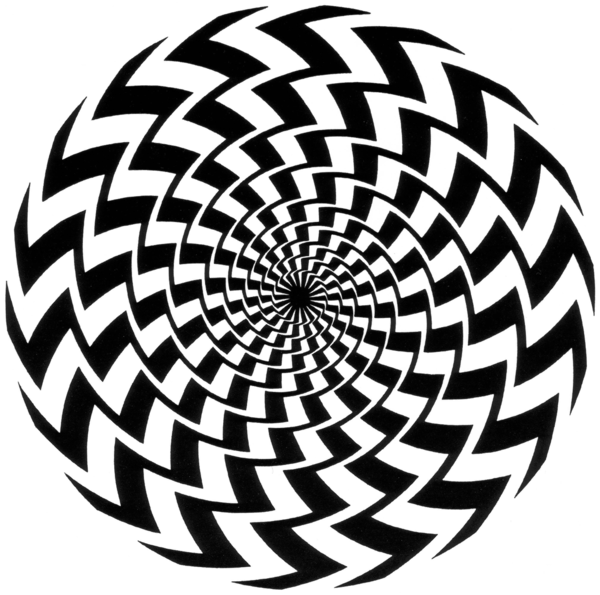
\includegraphics[width=0.93\linewidth]{./chapter/00.intro/pics/wadesSpirale.sm.png}};}
          \foreach \x in {20,16,12,9,4}{
            \only<3->{\draw[red,thick] (0,0) circle(\x mm);}
          }
        \else
          {\node at (0,0) {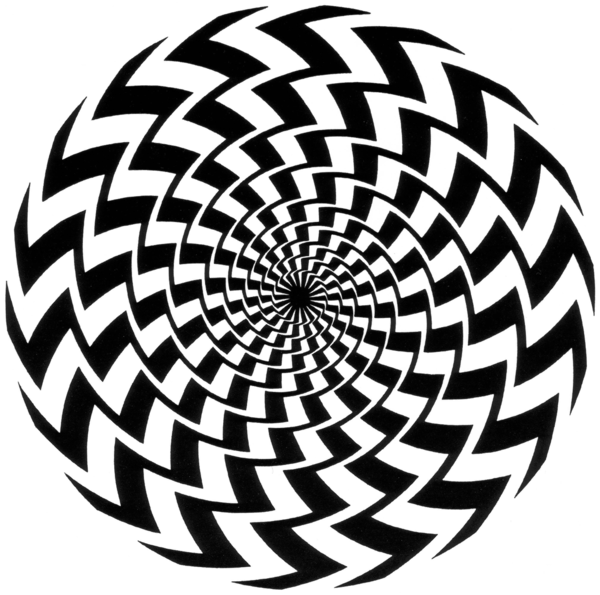
\includegraphics[width=0.93\linewidth]{./chapter/00.intro/pics/wadesSpirale.sm.png}};}
          % \foreach \x in {20,16,12,9,4}{
          %   {\draw[red,thick] (0,0) circle(\x mm);}
          % }
        \fi
      \end{tikzpicture}\\
      {\tiny from \cite[\tiny Apolin 2017, Big Bang 5 RG: \emph{1.1 Im Falle eines Falles}]{apolin2017:bigBang5RG}}
    }\hspace{\stretch{1}}\parbox[t]{0.62\linewidth}{
      \begin{itemize}
        \item <2-> Ist das eine Spirale? 
        \item <3-> \ifteacher Oder doch nur Kreise?
                   \else Zeichnen Sie Kreise ein.
                   \fi
        \item <5-> Die Behauptung (\ifteacher{}Hypothese\else \fbox{\phantom{Hypothese}}\fi),
          dass es eine \ifteacher Spirale \else \fbox{\phantom{Spirale}}\fi
          sei,  konnte widerlegt (\ifteacher{}falsifiziert\else \fbox{\phantom{falsifiziert}}\fi)
          werden.
      \end{itemize}
      \only<6->{\ifteacher In der Naturwissenschaftlichen Arbeitsweise werden
        \emph{Hypothesen} aufgestellt, die durch Experimente
        \emph{widerlegt} (falsifiziert) werden können.
        \else\fi}
    }
  \end{block}
  %%= = = = = = = = = = = = = = = = = = = = = = = = = = = = = = = = = = = = = =
\end{frame}
%==============================================================================

% \section{Intro}
% \subsection*{Naturwissenschaftliche Arbeitsweisen}
%= = = = = = = = = = = = = = = = = = = = = = = = = = = = = = = = = = = = = = =
%= = = = = = = = = = = = = = = = = = = = = = = = = = = = = = = = = = = = = = =
% \iffalse
\begin{frame}
  \frametitle{Naturwissenschaftliche Arbeitsweisen}
  \framesubtitle{Vom Fallen}
  %%= = = = = = = = = = = = = = = = = = = = = = = = = = = = = = = = = = = = = =
  \parbox[t]{0.2\linewidth}{\raisebox{\dimexpr-0.8\height+\ht\strutbox}{%%
    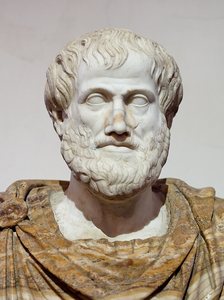
\includegraphics[width=0.99\linewidth]{./chapter/00.intro/pics/800px-Aristotle_Altemps_Inv8575.sm.png}}}
  \hspace{\stretch{1}}\parbox[t]{0.79\linewidth}{
    Lange Zeit glaubte man, dass schwere K\"orper schneller fallen als leichte
    (Aristoteles).
    Wie kann das \ifteacher{}widerlegt\else\fbox{\phantom{widerlegt}}\fi{}
    oder \ifteacher{}best\"atigt\else\fbox{\phantom{best\"atigt}}\fi{} werden?
    \\\vspace{\stretch{1}}
    {\tiny \cite[\url{https://upload.wikimedia.org/wikipedia/commons/a/ae/Aristotle_Altemps_Inv8575.jpg}]{enwiki:main}}
  }\\
  \pause
  \visible<+->{
    \begin{block}{Reales Experiment}
      \begin{itemize}
        \item<+-> Zwei Steine mit unterschiedlicher Masse werden
          \ifteacher{}gleichzeitig\else\fbox{\phantom{gleichzeitig}}\fi{}
          aus der \ifteacher{}gleichen\else\fbox{\phantom{gleichen}}\fi{}
          H\"ohe fallen gelassen.
        \item<+-> Durch \adSTField[1]{Beobachtung} beziehungsweise auch 
          \adSTField[2]{Messung} wird festgestellt, dass beide Steine
          \adSTField[2]{gleichenschnell} auf dem Boden aufkommen.
      \end{itemize}
    \end{block}
  }
  %%= = = = = = = = = = = = = = = = = = = = = = = = = = = = = = = = = = = = = =
\end{frame}
%==============================================================================

% \section{Intro}
% \subsection*{Naturwissenschaftliche Arbeitsweisen}
%= = = = = = = = = = = = = = = = = = = = = = = = = = = = = = = = = = = = = = =
%= = = = = = = = = = = = = = = = = = = = = = = = = = = = = = = = = = = = = = =
% \iffalse
\begin{frame}
  \frametitle{Naturwissenschaftliche Arbeitsweisen}
  \framesubtitle{Vom Fallen}
  %%= = = = = = = = = = = = = = = = = = = = = = = = = = = = = = = = = = = = = =
  
  Lange Zeit glaubte man, dass schwere K\"orper schneller fallen als leichte.
  Wie kann das \ifteacher{}widerlegt\else\fbox{\phantom{widerlegt}}\fi{}
  oder \ifteacher{}best\"atigt\else\fbox{\phantom{best\"atigt}}\fi{} werden?
  \pause
  \visible<+->{
    \begin{block}{Gedankenexperiment}
      \parbox[t]{0.3\linewidth}{
        \raisebox{\dimexpr-1.2\height+\ht\strutbox}{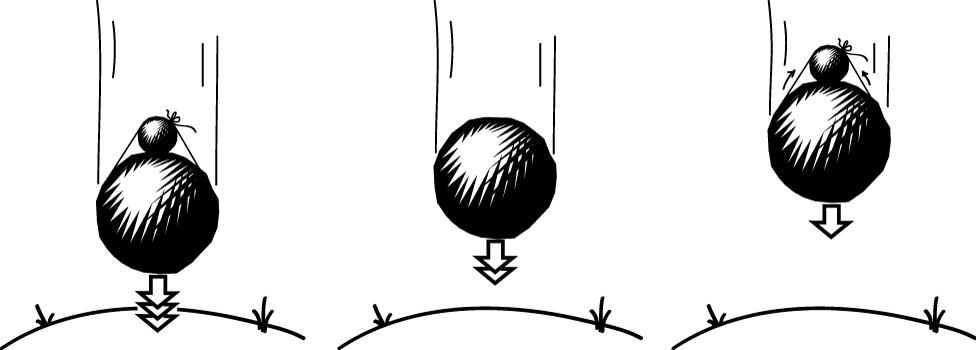
\includegraphics[width=0.98\linewidth]{./chapter/00.intro/pics/fallingStones.png}}\\
        {\tiny \url{https://personal.lse.ac.uk/robert49/ebooks/philsciadventures/img/balls2.gif}}
      }\hspace{\stretch{1}}\parbox[t]{0.69\linewidth}{
       \begin{itemize}
         \item<+-> \textbf{links}: Gro\ss{}er und kleiner Stein zusammen w\"urden
           \ifteacher{}schneller\else\fbox{\phantom{schneller}}\fi{}
           fallen (Aristoteles) als 
         \item<+-> \textbf{mitte}: der gro\ss{}e Stein alleine fallen w\"urde.
         \item <+-> \textbf{rechts}: der kleine Stein f\"allt laut Aristoteles
           \ifteacher{}langsamer\else\fbox{\phantom{langsamer}}\fi{} als der
           gro\ss{}e Stein, und w\"urde daher den gro\ss{}en Stein bremsen.
       \end{itemize}
      }
      \visible<+->{Das f\"uhrt zu einem \adSTField[1]{Widerspruch} zu Aristoteles,
      und veranlasste \adSTField[]{Galileo Galilei} zu der Annahme, dass
      alle K\"orper \adSTField[]{gleichschnell} fallen.}
    \end{block}
  }
  %%= = = = = = = = = = = = = = = = = = = = = = = = = = = = = = = = = = = = = =
\end{frame}
%==============================================================================

% \section{Intro}
% \subsection*{Naturwissenschaftliche Arbeitsweisen}
%= = = = = = = = = = = = = = = = = = = = = = = = = = = = = = = = = = = = = = =
%= = = = = = = = = = = = = = = = = = = = = = = = = = = = = = = = = = = = = = =
% \iffalse
\begin{frame}
  \frametitle{Naturwissenschaftliche Arbeitsweisen}
  \framesubtitle{Das Experiment}
  %%= = = = = = = = = = = = = = = = = = = = = = = = = = = = = = = = = = = = = =
  \parbox[t]{0.3\linewidth}{
    \raisebox{\dimexpr-1\height+\ht\strutbox}{%%
      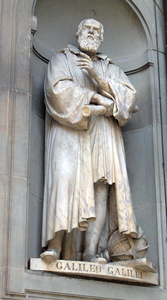
\includegraphics[width=0.75\linewidth]{./chapter/00.intro/pics/Galileo_Galilei01.sm.png}}\\
    {\tiny Von User:JoJan - Eigenes Werk, CC BY-SA 3.0, 
     \url{https://commons.wikimedia.org/w/index.php?curid=408982}
     \url{https://commons.wikimedia.org/wiki/File:Galileo_Galilei_2.jpg}}
  }\hspace{\stretch{1}}\parbox[t]{0.69\linewidth}{
  \adSTField[]{Galileo Galilei} f\"uhrte \adSTField[]{falsifizierbare} 
    Experimente ein, und begr\"undet damit die \adSTField[]{moderne 
    Naturwissenschaft}.
  \pause
  Aus einer \adSTField[2]{Behauptung} (Hypothese) wird ein
  \adSTField[2]{Experiment} abgeleitet, das die Hypothese
  \adSTField[2]{widerlegen} (falsifizieren) kann.\pause{} Wird durch 
  Experimente die Hypothese nicht widerlegt, so ist sie
  \adSTField[2]{best\"atigt}, aber nicht bewiesen, und wird 
  zu einer \adSTField[2]{Theorie} erhoben. 
  \pause 
  Von Galileo Galilei stammt auch der Ausspruch:
  \pause
  \begin{quote}
    {Alles, was messbar ist, messen, \\
    alles was nicht messbar ist, 
    messbar machen.}
  \end{quote}
  \pause 
  Nach \adSTField[1]{Sir Karl Raimund Popper} ist eine Theorie nur dann
  \adSTField[1]{wissenschaftlich}, wenn sie \adSTField[1]{falsifizierbar} ist.
 }
  %%= = = = = = = = = = = = = = = = = = = = = = = = = = = = = = = = = = = = = =
\end{frame}
%==============================================================================

\mode<beamer>{%%
% \section{Intro}
% \subsection*{Naturwissenschaftliche Arbeitsweisen}
%= = = = = = = = = = = = = = = = = = = = = = = = = = = = = = = = = = = = = = =
%= = = = = = = = = = = = = = = = = = = = = = = = = = = = = = = = = = = = = = =
% \iffalse
\begin{frame}
  \frametitle{Naturwissenschaftliche Arbeitsweisen}
  \framesubtitle{Reference}
  %%= = = = = = = = = = = = = = = = = = = = = = = = = = = = = = = = = = = = = =
{
\printbibliography[segment=\therefsegment,heading=subbib]
% \printbibliography[segment=\therefsegment,heading=subbibliography,title={Online Sources}]
}
\end{frame}
%==============================================================================
}

% % \section{Intro}
% \subsection*{Intro}
% %= = = = = = = = = = = = = = = = = = = = = = = = = = = = = = = = = = = = = = =
% %= = = = = = = = = = = = = = = = = = = = = = = = = = = = = = = = = = = = = = =
% % \iffalse
% \begin{frame}
%   \frametitle{Modelle}
%   \framesubtitle{Settings}
% %  \framesubtitle{Settings I}
%   %%= = = = = = = = = = = = = = = = = = = = = = = = = = = = = = = = = = = = = =
%
% \begin{block}{Settings I}
%   Die Kugeln werden nach der Ziehung
%   \begin{description}
%     \item [wieder zur\"uckgelegt]: der Ball kann daher \"ofter
%         gezogen werden, oder
%     \item [zur Seite gelegt]: dann wird der Ball maximal
%   einmal gezogen.
%   \end{description}
% \end{block}
%
% \pause
% \begin{block}{Settings II}
%   In der Urne befinden sich Kugeln, die
%   \begin{description}
%     \item [unterscheidbar sind]: jeder Ball ist ein Unikat (Farbe, Nummer,
%         Material, \dots)
%     \item [nicht unterscheidbar sind]: es gibt B\"alle, die die gleichen
%         Eigenschaften haben (z.~B. drei blaue und zwei rote B\"alle)
%   \end{description}
% \end{block}
%
% \end{frame}
% %==============================================================================
%
% % \section{Intro}
% % \subsection*{Modelle}
% %= = = = = = = = = = = = = = = = = = = = = = = = = = = = = = = = = = = = = = =
% %= = = = = = = = = = = = = = = = = = = = = = = = = = = = = = = = = = = = = = =
% % \iffalse
% \begin{frame}
%   \frametitle{Modelle}
%   \framesubtitle{Settings}
%   %%= = = = = = = = = = = = = = = = = = = = = = = = = = = = = = = = = = = = = =
%
% \begin{block}{Settings III}
%   Aus einer Urne mit $n$ Kugeln werden $k$ B\"alle gezogen.
%   \begin{description}
%     \item [$k=n$]: Permutationen
%     \item [$k<n$]: Variationen (alle B\"alle sind unterscheidbar)
%       und Kombinationen (B\"alle mit gleichen Eigenschaften)
%   \end{description}
% \end{block}
%
% \pause
% Aus wikipedia {\tiny(\url{https://de.wikipedia.org/wiki/Abz\%C3\%A4hlende_Kombinatorik\#Begriffsabgrenzungen})}:\\
% % https://de.wikipedia.org/wiki/Abz%C3%A4hlende_Kombinatorik#Begriffsabgrenzungen
% {\tiny
% Aufgrund der Vielfalt der Herangehensweisen sind die Schreibweisen und
% Begrifflichkeiten im Bereich der Kombinatorik leider oft recht uneinheitlich.
% Zwar bezeichnen übereinstimmend alle Autoren die Vertauschung der Reihenfolge
% einer Menge von $n$ unterscheidbaren Elementen als Permutation. W\"ahlt man
% dagegen von diesen $n$ Elementen nur $k < n$  Elemente aus, deren Reihenfolge
% man anschließend vertauscht, bezeichnen viele Autoren das nun als Variation,
% geordnete Stichprobe bzw. Kombination mit Berücksichtigung der Reihenfolge,
% andere dagegen (namentlich im englischsprachigen Raum) weiter als Permutation.
% L\"asst man schließlich in einer solchen Auswahl von Elementen deren
% Reihenfolge au\ss{}er Acht, wird solch eine Auswahl nun für gew\"ohnlich
% ungeordnete Stichprobe, Kombination ohne Berücksichtigung der Reihenfolge
% oder einfach nur Kombination genannt. Kombinationen sind also, sofern
% nichts weiter zu ihnen gesagt wird, in der Regel ungeordnet, Permutationen
% und/oder Variationen dagegen geordnet, wobei die Frage, ob man Permutationen
% als Sonderf\"alle von Variationen (oder umgekehrt) betrachtet, gegebenenfalls
% von Autor zu Autor unterschiedlich beantwortet wird.\\
% Alles in allem gibt es also zunächst einmal drei (oder auch nur zwei)
% verschiedene Fragestellungen, die ihrerseits noch einmal danach unterteilt
% werden, ob es unter den ausgewählten Elementen auch Wiederholungen gleicher
% Elemente geben darf oder nicht. Ist ersteres der Fall, spricht man von
% Kombinationen, Variationen oder Permutationen mit Wiederholung, andernfalls
% solchen ohne Wiederholung. Stellt man sich schließlich vor, dass die
% ausgew\"ahlten Elemente dabei einer Urne oder Ähnlichem entnommen werden,
% wird dementsprechend auch von Stichproben mit oder ohne Zur\"ucklegen
% gesprochen.\\
% }
%
% \end{frame}
% %==============================================================================

% $Header: svn+ssh://andre@crapman/home/junda/repos/andre/school/trunk/m/Chapter/stat/probability/chapter/prob.intro.tex 221 2021-02-13 18:18:09Z andre $
\tikzsetfigurename{ch.00.02.units}
% \tikzexternaldisable
% \tikzexternalenable

% \part{Kombi}
% \section{Intro}
\subsection*{\label{subsec0002.1_siUnit}SI-Einheiten}
%= = = = = = = = = = = = = = = = = = = = = = = = = = = = = = = = = = = = = = =
%= = = = = = = = = = = = = = = = = = = = = = = = = = = = = = = = = = = = = = =
% \iffalse
\begin{frame}
  \frametitle{SI-Einheiten}
  \framesubtitle{Das internationale Einheitensystem}
  %%= = = = = = = = = = = = = = = = = = = = = = = = = = = = = = = = = = = = = =
  \begin{block}{Messen - Gr\"o\ss{}en - Einheiten}
    \pause 
    Finden Sie heraus, wie folgende Einheiten definiert sind:\\
    \parbox[t]{0.30\linewidth}{
    \begin{itemize}
      \item <+-> Morgen (Fl\"ache)
      \item <+-> Elle (L\"ange)
      \item <+-> Meile (L\"ange)
      \item <+-> Pfund (Masse)
      \item <+-> Unze (Masse)
      \item <+-> Gallone (Volumen)
      \item <+-> Rie\ss{} (Volumen)
    \end{itemize}
    }\hspace{\stretch{1}}\parbox[t]{0.69\linewidth}{
    \ifteacher{%%
      \pause
      \begin{itemize}
        \item <+-> mit einem Ochsen am Vormittag pfl\"ugbare Fl\"ache
        \item <+-> Abstand Nase - Fingerspitze des
          gestreckten Arms
        \item <+-> u. a. 5000 Fuß, viele unterschiedliche Definitionen
        \item <+-> $\nicefrac{1}{2}$, 0,453\,592\,37 oder 373,241\,721\,6 kg
        \item <+-> $\nicefrac{1}{16}$ Pfund, 28,349\,523\,125 g
        \item <+-> 4,54609 l (UK), 3,78541 l (US)
        \item <+-> Menge Papier, die ein Esel tragen kann
           \\ heute: 480 oder 500 B\"ogen A4 Papier mit $\unitfrac[80]{g}{m^2}$
      \end{itemize}
    }
    \else{}\fi
    }
  \end{block}
  %%= = = = = = = = = = = = = = = = = = = = = = = = = = = = = = = = = = = = = =
\end{frame}
%==============================================================================

% \section{Intro}
% \subsection*{\label{subsec0002.1_siUnit}SI-Einheiten}
%= = = = = = = = = = = = = = = = = = = = = = = = = = = = = = = = = = = = = = =
%= = = = = = = = = = = = = = = = = = = = = = = = = = = = = = = = = = = = = = =
% \iffalse
\begin{frame}
  \frametitle{SI-Einheiten}
  \framesubtitle{Das internationale Einheitensystem}
  %%= = = = = = = = = = = = = = = = = = = = = = = = = = = = = = = = = = = = = =
  \begin{block}{Gr\"o\ss{}en und Einheiten}
    \pause 
    Physikalische Gr\"o\ss{}en sind messbare \adSTField[2]{Eigenschaften} von 
    Objekten, e. g. \adSTField[2]{L\"ange}, \adSTField[2]{Masse},
    \adSTField[2]{Zeit}, \adSTField[2]{Gewicht}, \adSTField[2]{elektrische
    Spannung}, \adSTField[2]{elektrische Stromst\"arke}, \dots
    \pause
    
    Physikalische \adSTField[2]{Einheiten} haben \adSTField[2]{definierte} 
    Werte f\"ur eine Gr\"o\ss{}e, z. B. \adSTField[2]{Meter} f\"ur
    \adSTField[2]{L\"ange}, \adSTField[2]{Kilogramm} f\"ur \adSTField[2]{Masse},
    \adSTField[2]{Sekunde} f\"ur \adSTField[2]{Zeit}, \dots
    
    \pause
    Mit genau definierten Einheiten k\"onnen Gr\"o\ss{}en an unterschiedlichen
    Orten und Zeiten \adSTField[2]{vergleichbar} gemacht werden. Manchmal 
    m\"ussen Gr\"o\ss{}en \adSTField[2]{umgerechnet} werden, z. B.
    \adSTField[2]{km/h} in \adSTField[2]{m/s}, oder \adSTField[2]{cm} in
    \adSTField[2]{Zoll}.

    \pause 
    Jede \adSTField[2]{Gr\"o\ss{}e} hat (mind.) ein \adSTField[2]{Symbol}, z. B.
    \adSTFieldm[2]{m} f\"ur \adSTField[2]{Masse}, \adSTFieldm[2]{t} f\"ur
    \adSTField[2]{Zeit}, \adSTFieldm[2]{F} f\"ur \adSTField[2]{Kraft}, \dots

    \pause 
    Jede \adSTField[2]{Einheit} hat auch eine Abk\"urzung, z. B.
    \adSTFieldm[2]{m} f\"ur \adSTField[2]{Meter}, \adSTFieldm[2]{s} f\"ur
    \adSTField[2]{Sekunde}, \adSTFieldm[2]{kg} f\"ur \adSTField[2]{Kilogramm}, \dots
  \end{block} 
  % \parbox[t]{0.2\linewidth}{
  % }\hspace{\stretch{1}}\parbox[t]{0.69\linewidth}{
  % }\\
  %%= = = = = = = = = = = = = = = = = = = = = = = = = = = = = = = = = = = = = =
\end{frame}
%==============================================================================

% \section{Intro}
% \subsection*{\label{subsec0002.1_siUnit}SI-Einheiten}
\ifteacher
%= = = = = = = = = = = = = = = = = = = = = = = = = = = = = = = = = = = = = = =
%= = = = = = = = = = = = = = = = = = = = = = = = = = = = = = = = = = = = = = =
% \iffalse
\begin{frame}
  \frametitle{SI-Einheiten}
  \framesubtitle{Das internationale Einheitensystem}
  %%= = = = = = = = = = = = = = = = = = = = = = = = = = = = = = = = = = = = = =
  \begin{block}{Vervollst\"andigen Sie die Tabelle}
    \pause 
    \begin{tabular}{@{}llll@{}}
      Gr\"o\ss{}e               & Symbol & Einheit   & Umrechnung \\ \hline
      L\"ange                   & $l$    & Meter     & 1 m = 100 cm = 1000 mm \\
      Masse                     & $m$    & Kilogramm & 1 kg = 1000 g = 1\,000\,000 mg \\
                                &        &           & 1 t = 1000 kg = 1\,000\,000 g \\
      Zeit                      & $t$    & Sekunde   & 1 min = 60 s; \\
                                &        &           & 1 h = 60 min = 3600 s \\
      L\"ange                   &  $l$  &  Meter      &  1 m  \\
      Masse       & $m$                &  Kilogramm  &  1 kg  \\
       Zeit        &  $t$  & Sekunde   &  1 s  \\
       Volumen     &  $V$  & Liter     &  1 L  \\
      Geschwindigkeit           &  $v$  &  Meter pro Sekunde  &  \unitfrac[1]{m}{s}  \\
       Beschleunigung  &  $a$  &  Meter pro Quadratsekunde  & $\unitfrac[1]{m}{s^2}$  \\
       Kraft          &  $F$  & Newton &  1 N \\
      elektrische Stromst\"arke & $I$    & Ampere    & 1 A = 1000 mA \\
      Temperatur                & $T$    & Kelvin    & K = ${^\circ}$C + 273,15 \\
      Stoffmenge                & $n$    & Mol       & mol\\
      Lichtst\"arke             & $J$    & Candela   & cd
    \end{tabular}
    
  \end{block}
  \parbox[t]{0.2\linewidth}{
  }\hspace{\stretch{1}}\parbox[t]{0.69\linewidth}{
  }\\
  %%= = = = = = = = = = = = = = = = = = = = = = = = = = = = = = = = = = = = = =
\end{frame}
%==============================================================================
\else
%= = = = = = = = = = = = = = = = = = = = = = = = = = = = = = = = = = = = = = =
% \iffalse
\begin{frame}
  \frametitle{SI-Einheiten}
  \framesubtitle{Das internationale Einheitensystem}
  %%= = = = = = = = = = = = = = = = = = = = = = = = = = = = = = = = = = = = = =
  \pause 
  \begin{block}{Vervollst\"andigen Sie die Tabelle}
    \begin{tabular}{@{}llll@{}}
      Gr\"o\ss{}e               & Symbol & Einheit   & Abk\"urzung \\ \hline
      L\"ange                   & \adSTField[2]{$l$} & \adSTField[2]{Meter}     & \adSTField[2]{1 m} \\
      \adSTField[2]{Masse}      & $m$                & \adSTField[2]{Kilogramm} & \adSTField[2]{1 kg} \\
      \adSTField[2]{Zeit}       & \adSTField[2]{$t$} & Sekunde   & \adSTField[2]{1 s} \\
      \adSTField[2]{Volumen}    & \adSTField[2]{$V$} & Liter     & \adSTField[2]{1 L} \\
      Geschwindigkeit           & \adSTField[2]{$v$} & \adSTField[2]{Meter pro Sekunde} & \adSTField[2]{\unitfrac[1]{m}{s}}\\
      \adSTField[2]{Beschleunigung} & \adSTField[2]{$a$} & \adSTField[2]{Meter pro Quadratsekunde} & \adSTFieldm[2]{\unitfrac[1]{m}{s^2}}\\
      \adSTField[2]{Kraft}         & \adSTField[2]{$F$} & Newton & \adSTField[2]{1 N} \\
      Temperatur                & \adSTField[2]{$T$}    & Kelvin    & K = ${^\circ}$C + 273,15 \\
    \end{tabular}
  \end{block}
  \parbox[t]{0.2\linewidth}{
    \ifteacher
      \rule[0pt]{0mm}{4\baselineskip}
    \else
      \rule[0pt]{0mm}{4\baselineskip}
    \fi

  }\hspace{\stretch{1}}\parbox[t]{0.69\linewidth}{
  }\\
  %%= = = = = = = = = = = = = = = = = = = = = = = = = = = = = = = = = = = = = =
\end{frame}
%==============================================================================
\fi

% \section{Intro}
% \subsection*{\label{subsec0002.1_siUnit}SI-Einheiten}
%= = = = = = = = = = = = = = = = = = = = = = = = = = = = = = = = = = = = = = =
%= = = = = = = = = = = = = = = = = = = = = = = = = = = = = = = = = = = = = = =
% \iffalse
\begin{frame}
  \frametitle{SI-Einheiten}
  \framesubtitle{Das internationale Einheitensystem}
  %%= = = = = = = = = = = = = = = = = = = = = = = = = = = = = = = = = = = = = =
    \pause
    \begin{block}{Einheitliche Einheiten}
    Das \adSTField[]{internationale Einheitensystem} (Système International
    d'Unités, SI) wurde 1960 von der 11. Generalkonferenz für Maß und Gewicht
    (CGPM) eingeführt, und ist heute das weltweit am meisten verwendete
    Einheitensystem. Es besteht aus sieben \adSTField[]{Basiseinheiten}, die
    alle anderen Einheiten lassen sich daraus ableiten.
    \pause
    \begin{itemize}
      \item <+-> Meter (m) - \adSTField[2]{L\"ange}
      \item <+-> Kilogramm (kg) - \adSTField[2]{Masse}
      \item <+-> Sekunde (s) - \adSTField[2]{Zeit}
      \item <+-> Ampere (A) - \adSTField[2]{elektrische Stromstärke}
      \item <+-> Kelvin (K) - \adSTField[2]{thermodynamische Temperatur}
      \item <+-> Mol (mol) - \adSTField[2]{Stoffmenge}
      \item <+-> Candela (cd) - \adSTField[2]{Lichtstärke}
    \end{itemize}
  \end{block} 
  \parbox[t]{0.2\linewidth}{
  }\hspace{\stretch{1}}\parbox[t]{0.69\linewidth}{
  }
  %%= = = = = = = = = = = = = = = = = = = = = = = = = = = = = = = = = = = = = =
\end{frame}
%==============================================================================

% \section{Intro}
\subsection*{\label{subsec0003.1_magnitude}Gr\"o\ss{}enordnungen}
%= = = = = = = = = = = = = = = = = = = = = = = = = = = = = = = = = = = = = = =
%= = = = = = = = = = = = = = = = = = = = = = = = = = = = = = = = = = = = = = =
% \iffalse
\begin{frame}
  \frametitle{Gr\"o\ss{}enordnungen}
  \framesubtitle{Prefixe und 10-er Potenzen}
  %%= = = = = = = = = = = = = = = = = = = = = = = = = = = = = = = = = = = = = =
  \begin{block}{Mikro bis Makro}
    \pause 
    \begin{itemize}
      \item <+-> Welche Masse besitzt die Erde? 
      \item <+-> Wie lang ist ein Lichtjahr? 
      \item <+-> Wie groß ist der Durchmesser eines Wasserstoffatoms?
      \item <+-> Wie viel wiegt ein Proton? 
      \item <+-> Wie lange dauert eine Nanosekunde?
    \end{itemize}
    \ifteacher
    \begin{itemize}
      \item <+-> 5\,970\,000\,000\,000\,000\,000\,000\,000 kg oder $5{,}97 \times 10^{24}$ kg 
      \item <+-> 9\,460\,000\,000\,000\,000 m oder $9{,}46 \times 10^{15}$ m 
      \item <+-> 0,000\,000\,000\,1 m oder $1 \times 10^{-10}$ m 
      \item <+-> 0,000\,000\,000\,000\,000\,000\,000\,000\,001\,67 kg $1{,}67 \times 10^{-27}$ kg 
      \item <+-> 0,000\,000\,001 s oder $1 \times 10^{-9}$ s 
    \end{itemize}
    }
    \else
    \rule[0pt]{0mm}{6\baselineskip}
    \fi
  \end{block} 
  \parbox[t]{0.2\linewidth}{
  }\hspace{\stretch{1}}\parbox[t]{0.69\linewidth}{
  }
  %%= = = = = = = = = = = = = = = = = = = = = = = = = = = = = = = = = = = = = =
\end{frame}
%==============================================================================

% \section{Intro}
% \subsection*{\label{subsec0003.1_magnitude}Gr\"o\ss{}enordnungen}
%= = = = = = = = = = = = = = = = = = = = = = = = = = = = = = = = = = = = = = =
%= = = = = = = = = = = = = = = = = = = = = = = = = = = = = = = = = = = = = = =
% \iffalse
\begin{frame}
  \frametitle{Gr\"o\ss{}enordnungen}
  \framesubtitle{Prefixe und 10-er Potenzen}
  %%= = = = = = = = = = = = = = = = = = = = = = = = = = = = = = = = = = = = = =
  \begin{block}{Von der Sch\"onheit von Zahlen}
    \pause
    Bei Gr\"o\ss{}en in der Natur kommen \adSTField[]{Zahlenwerte} vor, die mit
    vielen \adSTField[]{Nullen} dargestellt werden, und daher 
    \adSTField[2]{un\"ubersichtlich} sind. 
    \pause
    Man verwendet \adSTField[2]{10-er Potenzen}, um die Zahlen \"ubersichtlicher 
    anzuschreiben.
    \pause 
    Ebenso erleichern \adSTField[2]{Prefixe} die Lesbarkeit von Zahlen.
  \end{block} 
  \pause
  \begin{block}{10-er Potenzen}
    % \adRule{8}{5}%%
    \parbox[t]{0.23\linewidth}{%%
      \ifteacher%%
        \begin{array}[t]{@{}rrr@{}}
          n & 10^n & \text{Zahl}\tabularnewline
          \hline
          1 & 10^1 & 10 \tabularnewline
          2 & 10^2 & 100 \tabularnewline
          3 & 10^3 & 1000 \tabularnewline
          4 & 10^4 & 10\,000 \tabularnewline
          5 & 10^5 & 100\,000 \tabularnewline
            &&\dots\tabularnewline
          \hline
        \end{array}
      \else
        \begin{array}[t]{@{}rrr@{}}
          n & 10^n & \text{Zahl}\tabularnewline
          \hline
          1 & \fbox{\phantom{$10^1$}} & \fbox{\phantom{10      }} \tabularnewline
          2 & \fbox{\phantom{$10^2$}} & \fbox{\phantom{100     }} \tabularnewline
          3 & \fbox{\phantom{$10^3$}} & \fbox{\phantom{1000    }} \tabularnewline
          4 & \fbox{\phantom{$10^4$}} & \fbox{\phantom{10\,000 }} \tabularnewline
          5 & \fbox{\phantom{$10^5$}} & \fbox{\phantom{100\,000}} \tabularnewline
            &&\dots\tabularnewline
          \hline
        \end{array}
      \fi
    } 
    \ifteacher sowie \fi\pause
    \parbox[t]{0.23\linewidth}{%%
      \ifteacher%%
        \begin{array}[t]{@{}rrl@{}}
          n & 10^n & \text{Zahl}\tabularnewline
          \hline
          -1 & 10^{-1} & 0.1 \tabularnewline
          -2 & 10^{-2} & 0.01 \tabularnewline
          -3 & 10^{-3} & 0.001 \tabularnewline
          -4 & 10^{-4} & 0.000\,1 \tabularnewline
          -5 & 10^{-5} & 0.000\,01 \tabularnewline
            &&\dots\tabularnewline
          \hline
        \end{array}
      \else
        \begin{array}[t]{@{}rrr@{}}
          n & 10^n & \text{Zahl}\tabularnewline
          \hline
          -1 & \fbox{\phantom{$10^{-1}$}} & \fbox{\phantom{$0.1$}} \tabularnewline
          -2 & \fbox{\phantom{$10^{-2}$}} & \fbox{\phantom{$0.01$}} \tabularnewline
          -3 & \fbox{\phantom{$10^{-3}$}} & \fbox{\phantom{$0.001$}} \tabularnewline
          -4 & \fbox{\phantom{$10^{-4}$}} & \fbox{\phantom{$0.000\,1$}} \tabularnewline
          -5 & \fbox{\phantom{$10^{-5}$}} & \fbox{\phantom{$0.000\,01$}} \tabularnewline
            &&\dots\tabularnewline
          \hline
        \end{array}
      \fi
    } \pause
    \parbox[t]{0.42\linewidth}{%%
        Die Anzahl der \adSTField[2]{Nullen} in den 10-er Potenzen ist
        \begin{itemize}
          \item<+-> bei \adSTField[2]{positiven} Potenzen $n$ Nullen 
            nach der 1
          \item<+-> bei \adSTField[2]{negativen} Potenzen $n$ Nullen
            vor der 1, die Null vor dem Komma wird mitgez\"ahlt
        \end{itemize}
    }
  \end{block} 

  \parbox[t]{0.2\linewidth}{
  }\hspace{\stretch{1}}\parbox[t]{0.69\linewidth}{
  }
  %%= = = = = = = = = = = = = = = = = = = = = = = = = = = = = = = = = = = = = =
\end{frame}
%==============================================================================

% \section{Intro}
% \subsection*{\label{subsec0003.1_magnitude}Gr\"o\ss{}enordnungen}
%= = = = = = = = = = = = = = = = = = = = = = = = = = = = = = = = = = = = = = =
%= = = = = = = = = = = = = = = = = = = = = = = = = = = = = = = = = = = = = = =
% \iffalse
\begin{frame}
  \frametitle{Gr\"o\ss{}enordnungen}
  \framesubtitle{Prefixe und 10-er Potenzen}
  %%= = = = = = = = = = = = = = = = = = = = = = = = = = = = = = = = = = = = = =
  \begin{block}{Prefixe}
    \pause
    Prefixe sind Vorsilben, die vor eine Einheit gesetzt werden, um
    \adSTField[]{Vielfache} oder \adSTField[]{Bruchteile} dieser Einheit zu
    bezeichnen. 
    \pause
    Die Vielfachen und Bruchteile sind immer \adSTField[2]{Potenzen} von 10.
  \end{block} 
  \pause
  \begin{block}{Beispiele}
    \ifteacher{%%
    \begin{itemize}
      \item <+-> 1 Kilometer (km) = 1000 Meter (m) = $10^3$ m
      \item <+-> 1 Zentimeter (cm) = 0,01 Meter (m) = $10^{-2}$ m
      \item <+-> 1 Millisekunde (ms) = 0,001 Sekunden (s) = $10^{-3}$ s
      \item <+-> 1 Megahertz (MHz) = 1\,000\,000 Hertz (Hz) = $10^6$ Hz
      \item <+-> 1 Mikrogramm ($\mu$g) = 0,000\,001 Gramm (g) = $10^{-6}$ g
    \end{itemize}}
    \else
      \rule[0pt]{0mm}{8\baselineskip}
    \fi
  \end{block} 
  \parbox[t]{0.2\linewidth}{
  }\hspace{\stretch{1}}\parbox[t]{0.69\linewidth}{
  }
\end{frame}
%==============================================================================

% \section{Intro}
% \subsection*{\label{subsec0003.1_magnitude}Gr\"o\ss{}enordnungen}
%= = = = = = = = = = = = = = = = = = = = = = = = = = = = = = = = = = = = = = =
%= = = = = = = = = = = = = = = = = = = = = = = = = = = = = = = = = = = = = = =
% \iffalse
\begin{frame}
  \frametitle{Gr\"o\ss{}enordnungen}
  \framesubtitle{Prefixe und 10-er Potenzen}
  %%= = = = = = = = = = = = = = = = = = = = = = = = = = = = = = = = = = = = = =
  \begin{block}{Prefixe}
    \pause 
    \begin{tabular}{@{}l*{4}{@{\,}l}@{}}
      Name     & Symbol & Faktor       & 10-er       & Beispiel \tabularnewline
      &&&                                Potenz      &  \tabularnewline\hline
      Tera     & T      & 1\,000\,000\,000\,000 & $10^{12}$ & 1 TB = 1\,000\,000\,000\,000 B \tabularnewline
      Giga     & G      & 1\,000\,000\,000 & $10^{9}$      & 1 GHz = 1\,000\,000\,000 Hz \tabularnewline
      Mega     & M      & 1\,000\,000   & $10^{6}$            & 1 MW = 1\,000\,000 W \tabularnewline
      Kilo     & k      & 1\,000       & $10^3$            & 1 km = 1\,000 m \tabularnewline
      Hekto    & h      & 100         & $10^2$            & 1 hL = 100 L \tabularnewline
      Deka     & da     & 10          & $10^1$            & 1 dag = 10 g \tabularnewline
      (Einheit)&        & 1           & $10^0$            & 1 m = 1 m \tabularnewline
      Dezi     & d      & 0,1         & $10^{-1}$         & 1 dL = 0,1 L \tabularnewline
      Zenti    & c      & 0,01        & $10^{-2}$         & 1 cm = 0,01 m \tabularnewline
      Milli    & m      & 0,001       & $10^{-3}$         & 1 mg = 0,001 g \tabularnewline
      Mikro    & $\mu$  & 0,000\,001  & $10^{-6}$         & 1 $\mu$s = 0,000\,001 s \tabularnewline
      Nano     & n      & 0,000\,000\,001& $10^{-9}$      & 1 nm = 0,000\,000\,001 m \tabularnewline
      Pico     & p      & 0,000\,000\,000\,001& $10^{-12}$& 1 pF = 0,000\,000\,000\,001 F \tabularnewline
      % Femto    & f      & 0,000\,000\,000\,000\,001& $10^{-15}$& 1 fs = 0,000\,000\,000\,000\,001 s \tabularnewline
      % Atto     & a      & 0,000\,000\,000\,000\,000\,001& $10^{-18}$& 1 aJ = 0,000\,000\,000\,000\,000\,000\,001 J \tabularnewline
      % Zepto    & z      & 0,000\,000\,000\,000\,000\,000\,001& $10^{-21}$& 1 zW = 0,000\,000\,000\,000\,000\,000\,000\,000\,001 W \tabularnewline
      % Yocto    & y      & 0,000\,000\,000\,000\,000\,000\,000\,000\,000\,001& $10^{-24}$& 1 yC = 0,000\,000\,000\,000\,000\,000\,000\,000\,000\,000\,000\,001 C \tabularnewline
      \hline
    \end{tabular}
  \end{block} 
  %%= = = = = = = = = = = = = = = = = = = = = = = = = = = = = = = = = = = = = =
\end{frame}
%==============================================================================

% \section{Intro}
% \subsection*{Naturwissenschaftliche Arbeitsweisen}
%= = = = = = = = = = = = = = = = = = = = = = = = = = = = = = = = = = = = = = =
%= = = = = = = = = = = = = = = = = = = = = = = = = = = = = = = = = = = = = = =
% \iffalse
\begin{frame}
  \frametitle{Naturwissenschaftliche Arbeitsweisen}
  \framesubtitle{Vom Fallen}
  %%= = = = = = = = = = = = = = = = = = = = = = = = = = = = = = = = = = = = = =
  
  Lange Zeit glaubte man, dass schwere K\"orper schneller fallen als leichte.
  Wie kann das \ifteacher{}widerlegt\else\fbox{\phantom{widerlegt}}\fi{}
  oder \ifteacher{}best\"atigt\else\fbox{\phantom{best\"atigt}}\fi{} werden?
  \pause
  \visible<+->{
    \begin{block}{Gedankenexperiment}
      \parbox[t]{0.3\linewidth}{
        \raisebox{\dimexpr-1.2\height+\ht\strutbox}{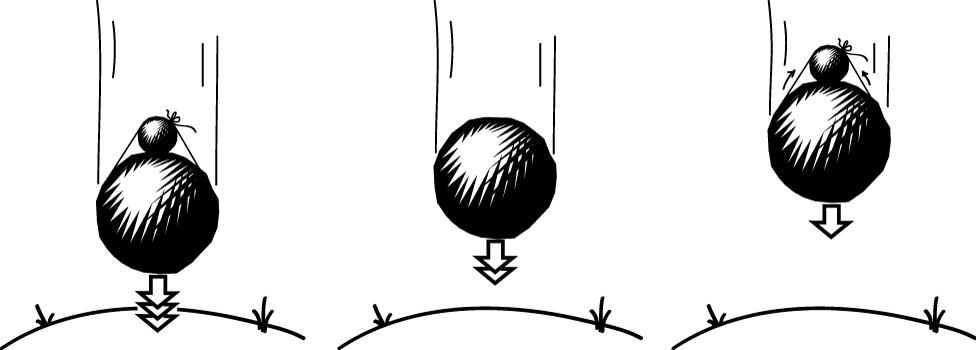
\includegraphics[width=0.98\linewidth]{./chapter/00.intro/pics/fallingStones.png}}\\
        {\tiny \url{https://personal.lse.ac.uk/robert49/ebooks/philsciadventures/img/balls2.gif}}
      }\hspace{\stretch{1}}\parbox[t]{0.69\linewidth}{
       \begin{itemize}
         \item<+-> \textbf{links}: Gro\ss{}er und kleiner Stein zusammen w\"urden
           \ifteacher{}schneller\else\fbox{\phantom{schneller}}\fi{}
           fallen (Aristoteles) als 
         \item<+-> \textbf{mitte}: der gro\ss{}e Stein alleine fallen w\"urde.
         \item <+-> \textbf{rechts}: der kleine Stein f\"allt laut Aristoteles
           \ifteacher{}langsamer\else\fbox{\phantom{langsamer}}\fi{} als der
           gro\ss{}e Stein, und w\"urde daher den gro\ss{}en Stein bremsen.
       \end{itemize}
      }
      \visible<+->{Das f\"uhrt zu einem \adSTField[1]{Widerspruch} zu Aristoteles,
      und veranlasste \adSTField[]{Galileo Galilei} zu der Annahme, dass
      alle K\"orper \adSTField[]{gleichschnell} fallen.}
    \end{block}
  }
  %%= = = = = = = = = = = = = = = = = = = = = = = = = = = = = = = = = = = = = =
\end{frame}
%==============================================================================

% \section{Intro}
% \subsection*{Naturwissenschaftliche Arbeitsweisen}
%= = = = = = = = = = = = = = = = = = = = = = = = = = = = = = = = = = = = = = =
%= = = = = = = = = = = = = = = = = = = = = = = = = = = = = = = = = = = = = = =
% \iffalse
\begin{frame}
  \frametitle{Naturwissenschaftliche Arbeitsweisen}
  \framesubtitle{Das Experiment}
  %%= = = = = = = = = = = = = = = = = = = = = = = = = = = = = = = = = = = = = =
  \parbox[t]{0.3\linewidth}{
    \raisebox{\dimexpr-1\height+\ht\strutbox}{%%
      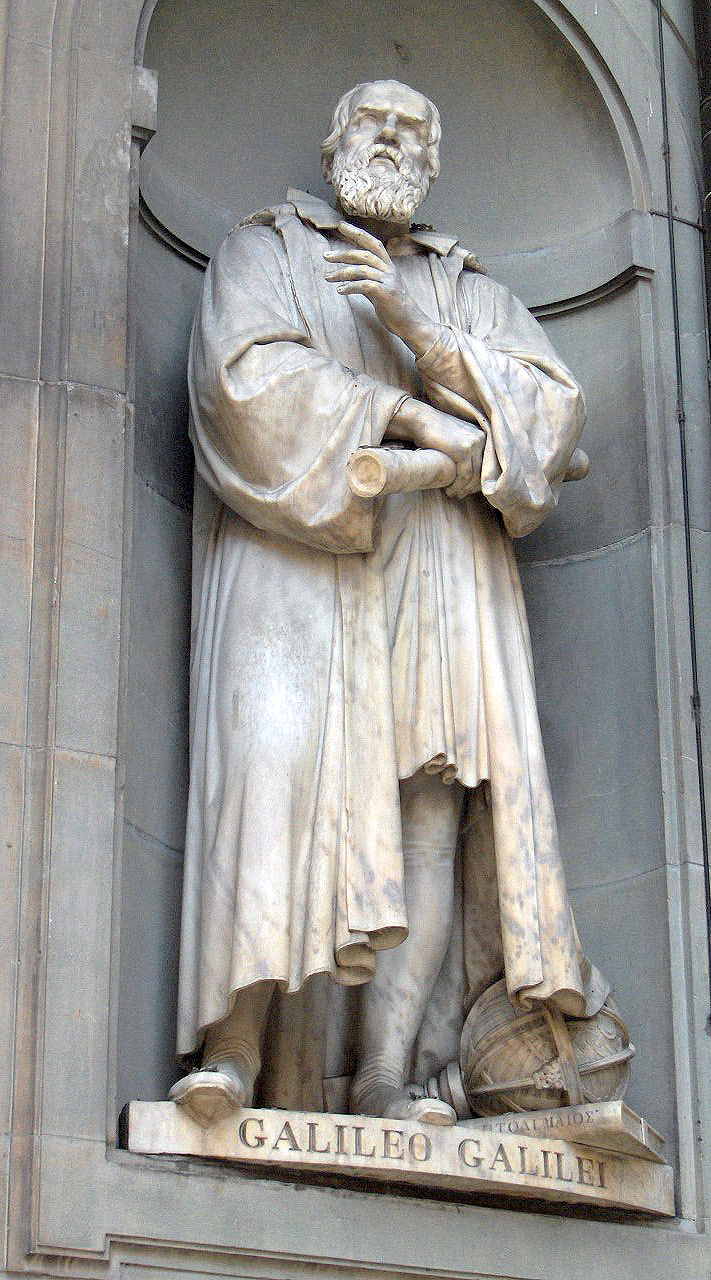
\includegraphics[width=0.75\linewidth]{./chapter/00.intro/pics/Galileo_Galilei01.png}}\\
    {\tiny Von User:JoJan - Eigenes Werk, CC BY-SA 3.0, 
     \url{https://commons.wikimedia.org/w/index.php?curid=408982}
     \url{https://commons.wikimedia.org/wiki/File:Galileo_Galilei_2.jpg}}
  }\hspace{\stretch{1}}\parbox[t]{0.69\linewidth}{
  \adSTField[]{Galileo Galilei} f\"uhrte \adSTField[]{falsifizierbare} 
    Experimente ein, und begr\"undet damit die \adSTField[]{moderne 
    Naturwissenschaft}.
  \pause
  Aus einer \adSTField[2]{Behauptung} (Hypothese) wird ein
  \adSTField[2]{Experiment} abgeleitet, das die Hypothese
  \adSTField[2]{widerlegen} (falsifizieren) kann.\pause{} Wird durch 
  Experimente die Hypothese nicht widerlegt, so ist sie
  \adSTField[2]{best\"atigt}, aber nicht bewiesen, und wird 
  zu einer \adSTField[2]{Theorie} erhoben. 
  \pause 
  Von Galileo Galilei stammt auch der Ausspruch:
  \pause
  \begin{quote}
    {Alles, was messbar ist, messen, \\
    alles was nicht messbar ist, 
    messbar machen.}
  \end{quote}
  \pause 
  Nach \adSTField[1]{Sir Karl Raimund Popper} ist eine Theorie nur dann
  \adSTField[1]{wissenschaftlich}, wenn sie \adSTField[1]{falsifizierbar} ist.
 }
  %%= = = = = = = = = = = = = = = = = = = = = = = = = = = = = = = = = = = = = =
\end{frame}
%==============================================================================

% % \section{Intro}
% % \subsection*{Naturwissenschaftliche Arbeitsweisen}
% %= = = = = = = = = = = = = = = = = = = = = = = = = = = = = = = = = = = = = = =
% %= = = = = = = = = = = = = = = = = = = = = = = = = = = = = = = = = = = = = = =
% % \iffalse
% \begin{frame}
%   \frametitle{Naturwissenschaftliche Arbeitsweisen}
%   \framesubtitle{Reference}
%   %%= = = = = = = = = = = = = = = = = = = = = = = = = = = = = = = = = = = = = =
% {
% \printbibliography[segment=\therefsegment,heading=subbib]
% % \printbibliography[segment=\therefsegment,heading=subbibliography,title={Online Sources}]
% }
% \end{frame}
% %==============================================================================

% % \section{Intro}
% \subsection*{Intro}
% %= = = = = = = = = = = = = = = = = = = = = = = = = = = = = = = = = = = = = = =
% %= = = = = = = = = = = = = = = = = = = = = = = = = = = = = = = = = = = = = = =
% % \iffalse
% \begin{frame}
%   \frametitle{Modelle}
%   \framesubtitle{Settings}
% %  \framesubtitle{Settings I}
%   %%= = = = = = = = = = = = = = = = = = = = = = = = = = = = = = = = = = = = = =
%
% \begin{block}{Settings I}
%   Die Kugeln werden nach der Ziehung
%   \begin{description}
%     \item [wieder zur\"uckgelegt]: der Ball kann daher \"ofter
%         gezogen werden, oder
%     \item [zur Seite gelegt]: dann wird der Ball maximal
%   einmal gezogen.
%   \end{description}
% \end{block}
%
% \pause
% \begin{block}{Settings II}
%   In der Urne befinden sich Kugeln, die
%   \begin{description}
%     \item [unterscheidbar sind]: jeder Ball ist ein Unikat (Farbe, Nummer,
%         Material, \dots)
%     \item [nicht unterscheidbar sind]: es gibt B\"alle, die die gleichen
%         Eigenschaften haben (z.~B. drei blaue und zwei rote B\"alle)
%   \end{description}
% \end{block}
%
% \end{frame}
% %==============================================================================
%
% % \section{Intro}
% % \subsection*{Modelle}
% %= = = = = = = = = = = = = = = = = = = = = = = = = = = = = = = = = = = = = = =
% %= = = = = = = = = = = = = = = = = = = = = = = = = = = = = = = = = = = = = = =
% % \iffalse
% \begin{frame}
%   \frametitle{Modelle}
%   \framesubtitle{Settings}
%   %%= = = = = = = = = = = = = = = = = = = = = = = = = = = = = = = = = = = = = =
%
% \begin{block}{Settings III}
%   Aus einer Urne mit $n$ Kugeln werden $k$ B\"alle gezogen.
%   \begin{description}
%     \item [$k=n$]: Permutationen
%     \item [$k<n$]: Variationen (alle B\"alle sind unterscheidbar)
%       und Kombinationen (B\"alle mit gleichen Eigenschaften)
%   \end{description}
% \end{block}
%
% \pause
% Aus wikipedia {\tiny(\url{https://de.wikipedia.org/wiki/Abz\%C3\%A4hlende_Kombinatorik\#Begriffsabgrenzungen})}:\\
% % https://de.wikipedia.org/wiki/Abz%C3%A4hlende_Kombinatorik#Begriffsabgrenzungen
% {\tiny
% Aufgrund der Vielfalt der Herangehensweisen sind die Schreibweisen und
% Begrifflichkeiten im Bereich der Kombinatorik leider oft recht uneinheitlich.
% Zwar bezeichnen übereinstimmend alle Autoren die Vertauschung der Reihenfolge
% einer Menge von $n$ unterscheidbaren Elementen als Permutation. W\"ahlt man
% dagegen von diesen $n$ Elementen nur $k < n$  Elemente aus, deren Reihenfolge
% man anschließend vertauscht, bezeichnen viele Autoren das nun als Variation,
% geordnete Stichprobe bzw. Kombination mit Berücksichtigung der Reihenfolge,
% andere dagegen (namentlich im englischsprachigen Raum) weiter als Permutation.
% L\"asst man schließlich in einer solchen Auswahl von Elementen deren
% Reihenfolge au\ss{}er Acht, wird solch eine Auswahl nun für gew\"ohnlich
% ungeordnete Stichprobe, Kombination ohne Berücksichtigung der Reihenfolge
% oder einfach nur Kombination genannt. Kombinationen sind also, sofern
% nichts weiter zu ihnen gesagt wird, in der Regel ungeordnet, Permutationen
% und/oder Variationen dagegen geordnet, wobei die Frage, ob man Permutationen
% als Sonderf\"alle von Variationen (oder umgekehrt) betrachtet, gegebenenfalls
% von Autor zu Autor unterschiedlich beantwortet wird.\\
% Alles in allem gibt es also zunächst einmal drei (oder auch nur zwei)
% verschiedene Fragestellungen, die ihrerseits noch einmal danach unterteilt
% werden, ob es unter den ausgewählten Elementen auch Wiederholungen gleicher
% Elemente geben darf oder nicht. Ist ersteres der Fall, spricht man von
% Kombinationen, Variationen oder Permutationen mit Wiederholung, andernfalls
% solchen ohne Wiederholung. Stellt man sich schließlich vor, dass die
% ausgew\"ahlten Elemente dabei einer Urne oder Ähnlichem entnommen werden,
% wird dementsprechend auch von Stichproben mit oder ohne Zur\"ucklegen
% gesprochen.\\
% }
%
% \end{frame}
% %==============================================================================

% \include{chapter/00.intro/ch.00.02.BasicPrinciples.tex}
\endrefsegment

% \include{chapter/ch01/prob.ch01.01.basics}
% \include{chapter/ch02/prob.ch02.prob.measure.01.intro}
% \include{chapter/ch02/prob.ch02.prob.measure.02.prob.distribution}
% \include{chapter/ch02/prob.ch02.prob.measure.06.prob.geometric}
% \include{chapter/ch02/prob.ch02.prob.measure.03.dist.binomial}
% \include{chapter/ch02/prob.ch02.prob.measure.04.dist.hypergeometric}
% \include{chapter/ch02/prob.ch02.prob.measure.05.dist.normal}
% \include{chapter/ch02/prob.ch02.prob.measure.05.dist.normal.applied}
% \include{chapter/ch01/prob.ch01.permutations.II}
% \include{chapter/ch01/prob.ch01.combinations}
% \include{chapter/ch01/prob.ch01.conclusion}
%
\iffalse
\else
\fi

%%= = = = = = = = = = = = = = = = = = = = = = = = = = = = = = = = = = = = = = =
%%= = = = = = = = = = = = = = = = = = = = = = = = = = = = = = = = = = = = = = =
%%\subsection{H\"oren}
\iffalse
\begin{frame}
  \frametitle{Die Kreisbewegung}
%%  \framesubtitle{H\"oren}
  % - A title should summarize the slide in an understandable fashion
  %   for anyone how does not follow everything on the slide itself.
%   %%= = = = = = = = = = = = = = = = = = = = = = = = = = = = = = = = = = = = = =
%   \begin{block}{Frequenz; (engl. frequency)}
%   Die Frequenz ist die Zahl der Schwingungen pro Sekunde.
%   Sie ist der Kehrwert der Periodendauer $T$.
%   \end{block}
%   %%= = = = = = = = = = = = = = = = = = = = = = = = = = = = = = = = = = = = = =
\begin{block}{Physikalische Beschreibung}
\begin{tabular}{c|c|c}
 L\"ange $s$	& Winkel $\varphi$ \\
 Geschwindigkeit $v$ & Winkelgeschwindigkeit $\omega$
		& Bahngeschwindigkeit \\
 $v=\frac{\Delta\,s}{\Delta\,t}$ & $\omega=\frac{\Delta\,\varphi}{\Delta\,t}$ & $v=\frac{2\,\pi\,r}{T}=\omega\,r$\\
 Beschleunigung & Winkelbeschleunigung $\alpha$ & Zentripedalbeschl. \\
 $a=\frac{\Delta\,v}{\Delta\,t}$ & $\alpha=\frac{\Delta\,\omega}{\Delta\,t}$ & $a=\frac{v^2}{r}=\omega{}^2\,r$\\
 		& $=0$ f\"ur gleichm\"a\ss{}ige \\
 		& Rotation
\end{tabular}
\parbox[b]{0.53\linewidth}{
\def\adang{30}
\begin{tikzpicture}[>={Stealth[length=5mm,round,open]}
        ,line cap=round,line join=round,inner sep=1,outer sep=2mm
        ,x=1.0cm,y=1.0cm,scale=3]
  \draw[line width=0.25mm] (0,0) coordinate (C) circle (0.1mm) node [left] {$C$}
        (0:1) coordinate (A) circle (0.1mm) node [right] {$A$}
        (\adang:1) coordinate (B) circle (0.1mm) node [right] {$B$};
  \draw [line width=0.35mm](C) + (-10:1) arc (-10:\adang+10:1);
  \draw [line width=0.35mm,->](C) -- node [pos=0.8,below] {$R$} (A);
  \draw [line width=0.35mm,->](C) -- node [pos=0.8,above] {$R$} (B);
  \draw [line width=0.35mm](C) + (0:0.3) node [below left] {$\Delta\,\varphi$} arc (0:\adang:0.3);
  \draw [line width=0.5mm,color=blue,->] (A) -- node [pos=0.6,right] {$v_A$} +(90:0.4);
  \draw [line width=0.5mm,color=blue,->] (B) -- node [pos=0.6,right] {$v_B$} +(90+\adang:0.4);
  \draw [line width=0.35mm,dashed](A) -- node [pos=0.6,left] {$\overline{S}$} (B);
\end{tikzpicture}
\begin{tikzpicture}[>={Stealth[length=5mm,round,open]}
        ,line cap=round,line join=round,inner sep=1,outer sep=2mm
        ,x=1.0cm,y=1.0cm,scale=3]
  \draw [line width=0.5mm,color=blue,->] (0,0) -- node [pos=0.6,right] {$v_A$} +(90:0.4) coordinate (AS);
  \draw [line width=0.5mm,color=blue,->] (0,0) -- node [pos=0.7,left] {$v_B$} +(90+\adang:0.4) coordinate (BS);
  \draw [line width=0.35mm,color=blue,outer sep=0mm] (0,0) +(90:0.2) arc (90:90+\adang:0.2) node [below left] {$\Delta\,\varphi$};
  \draw [line width=0.5mm,color=blue,->] (AS) -- node [pos=0.7,above] {$\Delta\,v$} (BS);
\end{tikzpicture}
}\hspace{\stretch{1}}\parbox[b]{0.46\linewidth}{\ \\[-1.2ex]
\footnotesize\noindent%%
$\begin{array}[b]{rcll}
  \text{Bogen } \widearc{S} &=& \varphi \cdot R\\
  \widearc{S} \approx \text{Sehne }\overline{S} \Rightarrow \varphi &=& \displaystyle\nicefrac{\overline{S}}{R}\\
  ABC \sim v_A v_B \Delta\,v &\multicolumn{2}{l}{\text{\"Ahnlichkeit}}\\
  \Rightarrow \displaystyle\nicefrac{\overline{S}}{R} &=& \displaystyle\nicefrac{\Delta\,v}{v}\\
  \Delta\,v &=& \displaystyle\nicefrac{\overline{S} \cdot v}{R} = \overline{S} \cdot \omega\\
  \nicefrac{\Delta\,v}{\Delta\,t} = \displaystyle\nicefrac{\omega \cdot \Delta\,\overline{S} }{\Delta\,t}
     &=& \displaystyle\nicefrac{ \omega \cdot R \cdot \Delta\,\varphi}{\Delta\,t} \\
     &=& \omega \cdot R \cdot \omega  \\
     &=& \omega^2 \cdot R
\end{array}$\\
Alternativ Differenzieren \\
in Polarkoordinaten mit $R=const.$.
}
\end{block}
\end{frame}

%%==============================================================================
% \section{Wiederholung Kreisbewegung}
%%\subsection{H\"oren}
%%= = = = = = = = = = = = = = = = = = = = = = = = = = = = = = = = = = = = = = =
\begin{frame}
  \frametitle{Schwingungen}
  %%----------------------------------------------------------------------------
  \begin{block}{Definitionen}
    Eine Schwingung ist ein periodischer Vorgang, bei der
    das schwingende System lokal an seinem Ort bleibt. Dabei
    schwanken Zustandsgr\"o\ss{}en eines Systems um einen Mittelwert
    (Federpendel, Herz, Spannung, Schweinzyklus, \dots).
    \begin{description}
      \item [Auslenkung] Momentane Gr\"o\ss{}e der Zustandsgr\"o\ss{}e
      \item [Amplitude $A$] maximale Auslenkung
      \item [Schwingungszyklus] vollst\"andige Hin- und Herbewegung
      \item [Periodendauer $T$] Zeit f\"ur einen Zyklus
      \item [Frequenz $f$] Anzahl der Zyklen pro Sekunde in $\si{Hz}$
	  \[
	  f=\frac{1}{T}
	  \]
    \end{description}
  \end{block}
  %%----------------------------------------------------------------------------
\end{frame}
%%= = = = = = = = = = = = = = = = = = = = = = = = = = = = = = = = = = = = = = =


%%==============================================================================
\section{Harmonische Schwingung}
\subsection{Federpendel}
%%= = = = = = = = = = = = = = = = = = = = = = = = = = = = = = = = = = = = = = =
\begin{frame}
  \frametitle{Federpendel; (engl. spring pendulum system?)}
%%  \framesubtitle{Schallquelle I; (engl. acoustic source)}
  % - A title should summarize the slide in an understandable fashion
  %   for anyone how does not follow everything on the slide itself.
  %%----------------------------------------------------------------------------
  \begin{block}{Schwingung einer Feder}
  \parbox{0.60\linewidth}{%%
  Die Auslenkung des Massest\"uckes $m$ um die Gleichgewichtslage $y=0$ f\"uhrt
  zu einer \"Anderung der Dehnung der Feder. Die \"Anderung der Federkraft
  folgt nach Hook:
  \[  \Delta F_y(y)=k\,y,\ \text{k \dots Federkonst. in \unitfrac{N}{m}  }  \]
  %\si[per-mode=fraction,fraction-function=\nicefrac]{\newton\per\meter}
  Die resultierende Kraft $F_\text{Res}$ bewirkt eine Beschleunigung $a$
  ($m\,a=\sum F$), und daraus die Bewegungsgleichungen der schwingende
  Masse:
  \[\begin{array}{rcll}
      m\,a_y&=&-k\,y\\
      m \frac{\diff{}^2 y}{\diff t^2} &=& -ky
  \end{array}\]
  }\hspace*{\stretch{1}}\parbox{0.38\linewidth}{%%
  \includegraphics[width=\linewidth]{federpendel}
  }\end{block}
  %%----------------------------------------------------------------------------

% \setbeamercolor{postit}{fg=black,bg=yellow}
% \begin{center}
% \begin{beamercolorbox}[sep=1em,wd=10cm,center]{postit}
% \usebeamerfont{title in head/foot}
% {\large
% $\Rightarrow${Die Ursache des Schalls sind Schwingungen.}}
% \end{beamercolorbox}
% \end{center}
\end{frame}
%%= = = = = = = = = = = = = = = = = = = = = = = = = = = = = = = = = = = = = = =

%%= = = = = = = = = = = = = = = = = = = = = = = = = = = = = = = = = = = = = = =
\begin{frame}
  \frametitle{Blick in die \emph{mathematische} Zukunft I}
  %%----------------------------------------------------------------------------
  \begin{block}{Gleichungssysteme}
    L\"osen von Gleichungssystemen $\rightarrow$ $n$ Variablen, $n$ Gleichungen\\
    es werden \emph{Zahlen} f\"ur die Variablen gesucht:
    \[\begin{array}{rcrcrcll}
        I &:& x &+& y &=& 4 \\
        II&:& x &-& y &=& 2 \\
        I+II &:& 2x && &=& 6 &\Rightarrow x=3\\
        && 3 &-& y &=& 2 &\Rightarrow y=1
      \end{array}
    \]
%   \parbox{0.60\linewidth}{%%
%
%   }\hspace*{\stretch{1}}\parbox{0.38\linewidth}{%%
%   \includegraphics[width=\linewidth]{federpendel}
%   }
  \end{block}
  %%----------------------------------------------------------------------------
\end{frame}
%%= = = = = = = = = = = = = = = = = = = = = = = = = = = = = = = = = = = = = = =

%%= = = = = = = = = = = = = = = = = = = = = = = = = = = = = = = = = = = = = = =
\begin{frame}
  \frametitle{Blick in die \emph{mathematische} Zukunft II}
  %%----------------------------------------------------------------------------
  \begin{block}{L\"osen von Differenzialgleichungen}
    L\"osen von Gleichungen, in denen Ableitungen von Funktionen
    vorkommen$\rightarrow$
    $f(x) = \text{irgendwas mit }f'(x)\text{ und/oder }f''(x)$:\\
    es werden \emph{Funktionen} f\"ur die \emph{Funktionsvariable} $f$ gesucht:
    \[\begin{array}{rcrcrcll}
        I &:& f(x) &=& \frac{1}{2}f'(x) &\rightarrow f(x)=?\\
      \end{array}\]
    Beim L\"osen werden Funktionen mittels Ansatz "ausprobiert":
    \[\begin{array}{rcrcrcll}
        \text{Ansatz} &:& f(x) &=& e^{ax}\\
        && f'(x) &=& a e^{ax} \\
        \text{Einsetzen} &:& e^{ax} &=& a\cdot\frac{1}{2}e^{ax} &| \div e^{ax}\\
        && 1 &=& a\cdot\frac{1}{2} &\Rightarrow a=2\\
        && f(x)&=&e^{2x}
      \end{array}\]
%   \parbox{0.60\linewidth}{%%
%
%   }\hspace*{\stretch{1}}\parbox{0.38\linewidth}{%%
%   \includegraphics[width=\linewidth]{federpendel}
%   }
  \end{block}
  %%----------------------------------------------------------------------------
\end{frame}
%%= = = = = = = = = = = = = = = = = = = = = = = = = = = = = = = = = = = = = = =

%%= = = = = = = = = = = = = = = = = = = = = = = = = = = = = = = = = = = = = = =
\begin{frame}
  \frametitle{Blick in die \emph{mathematische} Zukunft III}
  %%----------------------------------------------------------------------------
  \begin{block}{L\"osen von Differenzialgleichungen in der Form $\ddot{f}(t)+const. \cdot f(t)=0$}
    \[\begin{array}{rcrcrcll}
        \text{Ansatz} &:& f(t) &=& A \cdot \cos (\omega \cdot t + \phi)\\
        \text{oder} &:& f(t) &=& A \cdot \sin (\omega \cdot t + \phi)\\
      \end{array}\]
  {\footnotesize
    \[\begin{array}{r@{}c@{}rcrcll}
        && \frac{\diff}{\diff t} f(t) &=& - \omega A \cdot \sin (\omega \cdot t + \phi)\\
        && \frac{\diff{}^2}{\diff t^2} f(t) &=& -\omega{}^2 A \cdot \cos (\omega \cdot t + \phi)\\
        \text{Einsetzen} &:&
          -\omega{}^2 A \cdot \cos (\omega \cdot t + \phi) \quad\\
           &&\quad + const. \cdot A \cdot \cos (\omega \cdot t + \phi)
            &=& 0\\
          &&  (const.-\omega{}^2)\cdot A \cdot \cos (\omega \cdot t + \phi) &=& 0\\
      \Rightarrow && \omega{}^2 &=& const.\\
      \end{array}\]
  }
  $\omega$ wird durch die gegebene Konstante $const.$ bestimmt, die beiden
  neuen Variablen $\phi$ und $A$ sind aus dem physikalischem Kontext zu
  bestimmen (Anfangsbedingungen).
  \end{block}
  %%----------------------------------------------------------------------------
\end{frame}
%%= = = = = = = = = = = = = = = = = = = = = = = = = = = = = = = = = = = = = = =

%%= = = = = = = = = = = = = = = = = = = = = = = = = = = = = = = = = = = = = = =
\begin{frame}
  \frametitle{Federpendel}
%%  \framesubtitle{Schallquelle I; (engl. acoustic source)}
  %%----------------------------------------------------------------------------
  \begin{block}{L\"osung der Bewegungsgleichung}
  \parbox{0.48\linewidth}{%%
  \[\begin{array}{rcll}
    m\cdot a_y      &=& -k \cdot y\\
    m\cdot \ddot{y} &=& -k \cdot y\\
    \ddot{y} &=& - \frac{k}{m} \cdot y\\
    \ddot{y} + \frac{k}{m} \cdot y &=& 0\\
    \multicolumn{4}{r}{\text{Ansatz: }y = A \cos (\omega \cdot t + \phi)}\\
    \Rightarrow \omega{}^2 &=& \frac{k}{m}
  \end{array}\]
  }\hspace*{\stretch{1}}\parbox{0.48\linewidth}{%%
    \begin{tabular}{rcll}
      $\omega$ &\dots& \emph{Kreisfrequenz} \\
      && $\omega{} = 2 \pi f$\\
      $A$ &\dots & Amplitude \\
      $\phi$ & \dots & Phasenverschiebung
    \end{tabular}
  }\vspace{-3ex}
  %%----------------------------------------------------------------------------
    \begin{block}{Bsp. Federung eines Autos}
    \ \\[-6ex]
    \parbox[t]{0.48\linewidth}{%%
    \[\begin{array}{rrcrl}
      \text{Geg.} & m       &=& \unit[1\,000]{kg}\\
		  &m        &=& \unit[200]{kg}\\
		  &\Delta x &=& \unit[3]{cm}\\
    \end{array}\]
    }\hspace*{\stretch{1}}\parbox[t]{0.48\linewidth}{%%
    \[\begin{array}{rrcrl}
      \text{Ges.} & T       &=& \frac{1}{f}\\
		  & f	  &=& \frac{1}{\omega}\\
		  & \omega  &=& \sqrt{\frac{k}{m}} &= \sqrt{\frac{\frac{\Delta m\,g}{\Delta x}}{m}}
    \end{array}\]
    }
    \end{block}
  %%----------------------------------------------------------------------------
  \end{block}
\end{frame}
%%= = = = = = = = = = = = = = = = = = = = = = = = = = = = = = = = = = = = = = =

%%= = = = = = = = = = = = = = = = = = = = = = = = = = = = = = = = = = = = = = =
\begin{frame}
  \frametitle{Federpendel}
%%  \framesubtitle{Schallquelle I; (engl. acoustic source)}
  % - A title should summarize the slide in an understandable fashion
  %   for anyone how does not follow everything on the slide itself.
\begin{block}{Vom Kreis zum Pendel}
\definecolor{qqwuqq}{rgb}{0.,0.39215686274509803,0.}
\definecolor{ffqqqq}{rgb}{1.,0.,0.}
\definecolor{qqqqff}{rgb}{0.,0.,1.}
\definecolor{uuuuuu}{rgb}{0.26666666666666666,0.26666666666666666,0.26666666666666666}
\begin{tikzpicture}[>={Stealth[length=3mm,round,open]},scale=3/1,rotate=0
  ,outer sep=1mm,inner sep=0mm,line cap=round,line join=round,x=1.0cm,y=1.0cm]
\def\speed{0.8};
\def\acc{0.4};
\def\ang{50}
% \path ( $ cos(30)*(1,0) + sin(30)*(0,1) $ ) coordinate (A);
\path ( \ang:1 ) coordinate (A);
\draw[color=black,dashed] (0,0) -- (A);
\draw[color=black,dashed] (0.2,0.0) arc (0:\ang:0.2) node [right] {$\varphi$};

\draw[->,color=black] (-1.5,0.) -- (1.3,0.);
\foreach \x in {-1,1}
  \draw[shift={(\x,0)},color=black] (0pt,2pt) -- (0pt,-2pt) node[below] {\footnotesize $\x$};
\draw[->,color=black] (0.,-0.2) -- (0.,1.2);
\foreach \y in {1}
  \draw[shift={(0,\y)},color=black] (2pt,0pt) -- (-2pt,0pt) node[left] {\footnotesize $\y$};
\draw[color=black] (0pt,-10pt) node[right] {\footnotesize $0$};
\draw(-10:1) arc (-10:190:1);
\draw [->,line width=2.8pt,color=qqqqff]
  (A) circle(0.5pt) node [right] {$A$} ;
\draw [color=black,dashed] (A) +(90:0.2) arc (90:\ang+90:0.2) node [above,right] {$\varphi$};
\draw [->,line width=2.8pt,color=qqqqff,outer sep=1mm]
  (A) -- node[pos=0.7,below]{$v$} +(\ang+90:\speed);
\draw [->,line width=2.8pt,color=qqqqff,outer sep=1mm]
  (A) -- node[pos=0.7,right]{$v_y$} +($ cos(\ang)*(0,\speed) $);
\draw [->,line width=2.8pt,color=ffqqqq]
  (A) -- node[midway,left ]{$a$} ($ (A)!\acc!(0,0) $);
\draw [->,line width=2.8pt,color=ffqqqq]
  (A) -- node[pos=0.7,right]{$a_y$} +($ -sin(\ang)*(0,\acc) $);

\draw [->,line width=2.8pt,color=qqwuqq]
  (-1.5,0.) +($ sin(\ang)*(0,1) $)
  circle(0.5pt) node [right] {$B$};
\draw [->,line width=2.8pt,color=qqwuqq]
  (-1.5,0.) -- node[midway,right]{$y(t)$} +($ sin(\ang)*(0,1) $);


% \draw [->,line width=2.8pt,color=ffqqqq] (-0.36721993634590805,0.9301341399766526) -- (-1.0183138343295648,0.673080184534517);
% \draw [->,line width=2.8pt,color=ffqqqq] (-0.36721993634590805,0.9301341399766526) -- (-0.36721993634590805,0.673080184534517);
% \draw [->,line width=2.8pt,color=qqqqff] (-0.36721993634590805,0.9301341399766526) -- (-0.36721993634590805,0.4650670699883263);
% \begin{scriptsize}
% \draw [fill=black] (1.2258341817163252,1.0029629629629617) circle (2.5pt);
% \draw[color=black] (1.3385185185185182,1.1392592592592579) node {$phi = 8.23$};
% \draw[color=black] (-0.4866666666666657,0.7837037037037029) node {$c$};
% \draw [fill=uuuuuu] (A) circle (1.5pt);
% \draw [fill=uuuuuu] (-0.36721993634590805,0.9301341399766526) circle (1.5pt);
% \draw[color=uuuuuu] (-0.3266666666666658,1.0148148148148135) node {$A$};
% % \draw [fill=black] (0.5060818713450296,1.1807407407407393) circle (2.5pt);
% % \draw[color=black] (0.5859259259259262,1.3170370370370355) node {$phis = 2$};
% \draw[color=qqqqff] (-0.2259259259259251,0.7837037037037029) node {a};
% \draw[color=ffqqqq] (-0.6703703703703693,0.8251851851851842) node {v};
% \draw[color=ffqqqq] (-0.31481481481481394,0.8725925925925917) node {$v_y$};
% \draw[color=qqqqff] (-0.31481481481481394,0.7659259259259251) node {$a_y$};
% \draw[color=qqwuqq] (-1.9681481481481464,0.5170370370370365) node {$u$};
% \draw [fill=uuuuuu] (-2.,0.9301341399766526) circle (1.5pt);
% \draw[color=uuuuuu] (-1.9562962962962944,1.0148148148148135) node {$B$};
% \end{scriptsize}
\end{tikzpicture}

\parbox{0.5\linewidth}{%%
}\parbox{0.5\linewidth}{%%
}%%
\end{block}

\end{frame}
%%= = = = = = = = = = = = = = = = = = = = = = = = = = = = = = = = = = = = = = =

%%= = = = = = = = = = = = = = = = = = = = = = = = = = = = = = = = = = = = = = =
\begin{frame}
  \frametitle{Federpendel}
%%  \framesubtitle{Schallquelle I; (engl. acoustic source)}
  % - A title should summarize the slide in an understandable fashion
  %   for anyone how does not follow everything on the slide itself.
\begin{block}{Vom Kreis zum Pendel}
\begin{equation*}
\begin{aligned}
 y &= r\,\sin\varphi  &v_y&=v\,\cos\varphi  & a_y&=-a\,\sin\varphi  \\
 y &= r\,\sin\omega{}t &v_y&=\omega\,r\,\cos\omega{}t & a_y&=-\omega^2\,r\,\sin\omega{}t  \\
\end{aligned}
\end{equation*}
Daher
\[
 -\omega^2\,r\,\sin\omega{}t=-\frac{k}{m}\,\sin\omega{}t
\]
und daraus ergibt sich f\"ur $\omega=\sqrt\frac{k}{m}$ und
f\"ur die Periodendauer:
\[
 T=2\pi\,\sqrt{\frac{m}{k}}
\]

\parbox{0.5\linewidth}{%%
}\parbox{0.5\linewidth}{%%
}%%
\end{block}

\end{frame}
%%= = = = = = = = = = = = = = = = = = = = = = = = = = = = = = = = = = = = = = =

%%= = = = = = = = = = = = = = = = = = = = = = = = = = = = = = = = = = = = = = =
\begin{frame}
  \frametitle{Harmonische Schwingung, harmonischer Oszilator}
%%  \framesubtitle{Schallquelle I; (engl. acoustic source)}
  %%----------------------------------------------------------------------------
  \begin{block}{Definition}
    Jedes System, bei dem die resultierende R\"uckstellgr\"o\ss{}e
    (Kraft) direkt pro\-port\-ional zur Auslenkung ist, f\"uhrt zu einer
    harmonischen Schwingung.
  %%----------------------------------------------------------------------------
    \begin{block}{Beispiele}
      \begin{tabular}[t]{|*{5}{p{1.98cm}|}}
	\hline
	Federpendel & Fadenpendel & Drehpendel & Physisches & Fl\"ussigkeit\\
	\hline\hline
	Masse $m$   & Widerstands\-mom. $m \cdot l^2$   & Widerstands\-moment $J$
					      &Widerstands\-moment $J$
							    & Masse $m$ $=\rho \cdot A \cdot L$ \\
	\hline
	$\Delta\,x$ & $\Delta\,\varphi$
				  & $\Delta\,\varphi$
					      & $\Delta\,\varphi$
							    & $\Delta\,h$\hspace{\stretch{1}}\\
	\hline
	Kraft $k\cdot \Delta\,x$
		    & Drehmoment \linebreak $m \cdot g \cdot l \cdot \sin \varphi$
				& Drehmoment   $M=$ $k^{\star} \cdot \Delta\,\varphi$
					      & Drehmoment   $m \cdot g \cdot s \cdot \sin \varphi$
							    & Kraft \par$\rho \cdot A \cdot g \cdot 2\Delta\,h$\\
	\hline
	$T = 2\pi\,\sqrt{\frac{m}{k}}$
		    & $2\pi\sqrt{\frac{l}{g}}$
				& $2\pi\sqrt{\frac{J}{k^{\star}}}$
					      & $2\pi\sqrt{\frac{J}{m\,g\,s}}$
							  & $2\pi\sqrt{\frac{L}{2g}}$\\
	\hline
      \end{tabular}
%       \begin{description}
% 	\item [Drehpendel] Auslenkung: $\varphi$, R\"uckstellgr\"o\ss{}e $M$,
%
%       \end{description}

    \end{block}
  %%----------------------------------------------------------------------------
  \end{block}
\end{frame}
%%= = = = = = = = = = = = = = = = = = = = = = = = = = = = = = = = = = = = = = =

%==============================================================================
% \section{Harmonische Schwingung}
\subsection{Mathematisches Pendel}
%%= = = = = = = = = = = = = = = = = = = = = = = = = = = = = = = = = = = = = = =
\begin{frame}
  \frametitle{Mathematisches Pendel oder Fadenpendel I}
%%  \framesubtitle{Schallquelle I; (engl. acoustic source)}
  % - A title should summarize the slide in an understandable fashion
  %   for anyone how does not follow everything on the slide itself.
\begin{block}{Betrachtungen im Translationssystem}
\parbox{0.23\linewidth}{%%
\begin{tikzpicture}[>={Stealth[length=3mm,round,open]},scale=4/1,rotate=0
  ,outer sep=1mm,inner sep=0mm,line cap=round,line join=round,x=1.0cm,y=1.0cm]
\def\FG{0.5};
\def\acc{0.4};
\def\ang{20}
\draw[line width=0.7mm] (0,0) -- ($ (0,0)!0.90!(\ang-90:1) $);
\draw[line width=0.7mm,outer sep=0.25] (\ang-90:1) coordinate (M)
  node [outer sep=1mm,above] {$m$} circle (0.1) ;
\draw[line width=0.35mm,dashed] (M) arc (\ang-90:-90:1) ;
\draw[line width=0.35mm,dashed] (0,0) -- ($ (0,0)!0.90!(-90:1) $);
\draw[line width=0.35mm,dashed] (-90:1) coordinate (M0) circle (0.1);
\draw[line width=0.35mm,dashed] (-90:0.2) arc (-90:\ang-90:0.2)
  node [below left,fill=white] {$\varphi (t)$};
\draw[line width=1mm,->,blue] (M) -- +(0,-\FG)
  coordinate (FGe) node [right] {$F_\mathrm{G}$};
\draw[line width=1mm,->,green] (M) -- +(\ang-180:{sin(\ang)*\FG})
  coordinate (FRe) node [above] {$F_\mathrm{R}$};
\draw[line width=1mm,->,red] (M) -- +(\ang:{sin(\ang)*\FG})
  node [pos=0.7,outer sep=2mm,below] {$m\cdot\vec{a}$} coordinate (Fa) ;
\draw[line width=0.35mm,dashed] (FGe) -- (FRe);
\draw[line width=0.35mm,dashed] (FGe) +(90:0.2) arc (90:\ang+90:0.2) ;
\draw[line width=0.35mm,dashed] (M) arc (90:\ang+90:0.2) ;
\begin{scope}[rotate=\ang]
  \draw[shift={(0.2,0.0)},<->] (0,0) -- +(-90:1)
    node [midway,right]{$l$};
  \draw[] (0,0) -- +(0.21,0);
  \draw[] (-90:1) -- +(0.21,0);
\end{scope}

\end{tikzpicture}
}\hspace{\stretch{1}}\parbox{0.77\linewidth}{%%
\begin{tabular}[t]{r@{\,\dots}l}
 $\varphi(t)$ & Elongation \\
 $m$         & Masse \\
 $F_\mathrm{G}$& Gewichtskraft\\
 $F_\mathrm{R}$& R\"uckstellkraft \\
 $l$         & Fadenl\"ange
\end{tabular}\\[2ex]
{%\footnotesize
\begin{array}[t]{rcll}
   F_\mathrm{R} &=& F_\mathrm{G} \cdot \sin \varphi(t) &| \varphi \ll 1 \Rightarrow \\
   		&=& F_\mathrm{G} \cdot \varphi(t) &| \sin \varphi \approx  \varphi \\
   		&=& m \cdot g \cdot \varphi(t)    &| \text{f\"ur } \varphi \text{ in Radiant}\\
   		&\sim & \varphi(t) = const. \cdot \varphi(t) \\[1.5ex]
   F_\mathrm{R} &=& -m \cdot a(t) &| \text{Winkelbeschleunigung }\\
 		&=& -m \cdot \frac{\diff^2}{\diff\,t^2}{(l \cdot \varphi(t))}
				  &| b = \varphi \cdot l, a = \alpha \cdot l\\
   		&=& -m \cdot l \cdot \ddot{\varphi}(t) \quad
   		    &| \alpha = \cdot l \ddot{\varphi}(t)\\
   	       (&=&  -m \cdot l \cdot \alpha(t))
\end{array}
}
}%%
\end{block}
\end{frame}
%%= = = = = = = = = = = = = = = = = = = = = = = = = = = = = = = = = = = = = = =

%==============================================================================
% \section{Harmonische Schwingung}
% \subsection{Mathematisches Pendel}
%%= = = = = = = = = = = = = = = = = = = = = = = = = = = = = = = = = = = = = = =
\begin{frame}
  \frametitle{Mathematisches Pendel oder Fadenpendel II}
\begin{block}{Betrachtungen im Rotationssystem}
\parbox{0.23\linewidth}{%%
\begin{tikzpicture}[>={Stealth[length=3mm,round,open]},scale=4/1,rotate=0
  ,outer sep=1mm,inner sep=0mm,line cap=round,line join=round,x=1.0cm,y=1.0cm]
\def\FG{0.5};
\def\acc{0.4};
\def\ang{20}
\draw[line width=0.7mm] (0,0) -- ($ (0,0)!0.90!(\ang-90:1) $);
\draw[line width=0.7mm,outer sep=0.25] (\ang-90:1) coordinate (M)
  node [outer sep=1mm,above] {$m$} circle (0.1) ;
\draw[line width=0.35mm,dashed] (M) arc (\ang-90:-90:1) ;
\draw[line width=0.35mm,dashed] (0,0) -- ($ (0,0)!0.90!(-90:1) $);
\draw[line width=0.35mm,dashed] (-90:1) coordinate (M0) circle (0.1);
\draw[line width=0.35mm,dashed] (-90:0.2) arc (-90:\ang-90:0.2)
  node [below left,fill=white] {$\varphi (t)$};
\draw[line width=1mm,->,blue] (M) -- +(0,-\FG)
  coordinate (FGe) node [right] {$F_\mathrm{G}$};
\draw[line width=1mm,->,green] (M) -- +(\ang-180:{sin(\ang)*\FG})
  coordinate (FRe) node [above] {$F_\mathrm{R}$};
\draw[line width=1mm,->,red] (M) -- +(\ang:{sin(\ang)*\FG})
  node [pos=0.7,outer sep=2mm,below] {$m\cdot\vec{a}$} coordinate (Fa) ;
\draw[line width=0.35mm,dashed] (FGe) -- (FRe);
\draw[line width=0.35mm,dashed] (FGe) +(90:0.2) arc (90:\ang+90:0.2) ;
\draw[line width=0.35mm,dashed] (M) arc (90:\ang+90:0.2) ;
\begin{scope}[rotate=\ang]
  \draw[shift={(0.2,0.0)},<->] (0,0) -- +(-90:1)
    node [midway,right]{$l$};
  \draw[] (0,0) -- +(0.21,0);
  \draw[] (-90:1) -- +(0.21,0);
\end{scope}

\end{tikzpicture}
}\hspace{\stretch{1}}\parbox{0.77\linewidth}{%%
\begin{tabular}[t]{r@{\,\dots}l}
 $\varphi(t)$ & Elongation \\
 $m$         & Masse \\
 $F_\mathrm{G}$& Gewichtskraft\\
 $F_\mathrm{R}$& R\"uckstellkraft \\
 $l$         & Fadenl\"ange
\end{tabular}\\[2ex]
{%\footnotesize
\begin{array}[t]{rcll}
   M_\mathrm{R} &=& F_\mathrm{G} \cdot l \cdot \sin \varphi(t) &| \varphi \ll 1 \Rightarrow \\
   		&=& F_\mathrm{G} \cdot l \cdot \varphi(t) &| \sin \varphi \approx  \varphi \\
   		&=& m \cdot g \cdot l \cdot \varphi(t)    &| \text{f\"ur } \varphi \text{ in Radiant}\\
   		&\sim & \varphi(t) = const. \cdot \varphi(t) \\[1.5ex]
   M_\mathrm{R} &=& -J \cdot \alpha(t) &| \text{Winkelbeschleunigung }\\
 		&=& -m \cdot l^2 \cdot \ddot{\varphi}(t)
\end{array}
}
}%%
\end{block}
\end{frame}
%%= = = = = = = = = = = = = = = = = = = = = = = = = = = = = = = = = = = = = = =

%%= = = = = = = = = = = = = = = = = = = = = = = = = = = = = = = = = = = = = = =
\begin{frame}
  \frametitle{Mathematisches Pendel oder Fadenpendel III}
%%  \framesubtitle{Schallquelle I; (engl. acoustic source)}
  % - A title should summarize the slide in an understandable fashion
  %   for anyone how does not follow everything on the slide itself.
\begin{block}{L\"osung der Diffgleichung}
Die R\"uckstellkraft / das R\"uckstellmoment ist
proportional der Auslenkung $\varphi$ $\Rightarrow$ es
handelt sich um eine harmonische Schwingung (in der ersten N\"aherung).
\begin{array}[t]{rclrcl}
   F_\mathrm{R} &=& m \cdot g \cdot \varphi(t)
                         & M_\mathrm{R} &=& m \cdot g \cdot l \cdot \varphi(t)\\
   F_\mathrm{R} = -m \cdot \vec{a} &=& -m \cdot l \cdot \ddot{\varphi}(t)
      & M_\mathrm{R} = -J \cdot \alpha(t) &=& -m \cdot l^2 \cdot \ddot{\varphi}(t)\\
   \cancel{m} \cdot g \cdot \varphi(t) &=& - \cancel{m} \cdot l \cdot \ddot{\varphi}(t)
   & \quad\quad\cancel{m} \cdot \cancel{l} \cdot g \cdot \varphi(t) &=&
     -\cancel{m} \cdot l^{\cancel{2}} \cdot \ddot{\varphi}(t)\\[1.5ex]

   g \cdot \varphi(t) &=& -l \cdot \ddot{\varphi}(t) &\multicolumn{3}{l}{| \div l; + \ddot{\varphi}(t) }\\
   \frac{g}{l} \cdot \varphi(t)  + \ddot{\varphi}(t) &=& 0
                                             &\multicolumn{3}{l}{| \text{Diffgleichung in }\varphi(t)} \\[1.5ex]
   \omega &=&  \frac{g}{l} &\multicolumn{3}{l}{| \omega	= 2 \pi f = \frac{2 \pi}{T} } \\[2ex]
   f &=& \frac{1}{2\pi}\sqrt{\frac{g}{l}} & \quad T &=& 2\pi \sqrt{\frac{l}{g}} \\
\end{array}

\end{block}

\end{frame}
%%= = = = = = = = = = = = = = = = = = = = = = = = = = = = = = = = = = = = = = =

%%= = = = = = = = = = = = = = = = = = = = = = = = = = = = = = = = = = = = = = =
\begin{frame}
  \frametitle{Mathematisches Pendel oder Fadenpendel IV}
%%  \framesubtitle{Schallquelle I; (engl. acoustic source)}
  % - A title should summarize the slide in an understandable fashion
  %   for anyone how does not follow everything on the slide itself.
\begin{block}{Betrachtungen im Rotationssystem}
Die R\"uckstellkraft ist
proportional der Auslenkung $\varphi$ $\Rightarrow$ es
handelt sich um eine harmonische Schwingung (in der ersten N\"aherung).
\begin{array}[t]{rcll}
   F_\mathrm{R} &=& m \cdot g \cdot \varphi(t)   \\
   F_\mathrm{R} = -m \cdot \vec{a} &=& -m \cdot l \cdot \ddot{\varphi}(t) \\[1.5ex]
   \cancel{m} \cdot g \cdot \varphi(t) &=& - \cancel{m} \cdot l \cdot \ddot{\varphi}(t)
                                             &| \div l + \ddot{\varphi}(t) \\
   \frac{g}{l} \cdot \varphi(t)  + \ddot{\varphi}(t) &=& 0
                                             &| \text{Diffgleichung in }\varphi(t) \\[1.5ex]
   \omega	&=& \sqrt{\frac{g}{l}}	     &| \omega = 2 \pi f = \frac{2 \pi}{T} \\
   f &=& \frac{1}{2\pi}\sqrt{\frac{g}{l}} \\
   T &=& 2\pi \sqrt{\frac{l}{g}} \\
\end{array}

\end{block}

\end{frame}
%%= = = = = = = = = = = = = = = = = = = = = = = = = = = = = = = = = = = = = = =

%==============================================================================
% \section{Harmonische Schwingung}
\subsection{Widerstandsmoment}
%%= = = = = = = = = = = = = = = = = = = = = = = = = = = = = = = = = = = = = = =
\begin{frame}
  \frametitle{Tr\"agheitsmoment}
%%  \framesubtitle{Schallquelle I; (engl. acoustic source)}
  % - A title should summarize the slide in an understandable fashion
  %   for anyone how does not follow everything on the slide itself.
\begin{block}{Massentr\"agheitsmoment $J$ \hspace*{\stretch{1}}polares \\
                  \hspace*{\stretch{1}} Fl\"achentr\"agheitsmoment $I_p$}
\parbox[t]{0.48\linewidth}{
\begin{array}[t]{rcll}
   J &=& \sum\limits_{i=1}^n m_i \cdot r_i^2 \\
     &=& \sum A_i\,h_i\,\rho \cdot r_i^2 &| \text{f\"ur ebene}\\
     &=& h\,\rho \sum A_i \cdot r_i^2    &| \text{K\"orper}\\
     &=& h\,\rho I_p
\end{array}
}\hspace{\stretch{1}}\parbox[t]{0.48\linewidth}{
\begin{array}[t]{rcll}
   I_p &=& \sum\limits_{i=1}^n r_i^2 \cdot A_i\\
   \multicolumn{4}{r}{\text{einfach mittels Integral zu berechnen}}\\
   \multicolumn{4}{r}{\text{siehe Sommersemester Mathe}}\\
   I_p &=& I_y + I_z &(=\sum A_i \cdot (y_i\mid z_i)^2)
\end{array}
}
\begin{block}{Beispiele}
\begin{tabular}[t]{ccc}
  Rechteck & Dreieck & Kreisring und Kreis ($r=0$)\\
  \tikz[>={Stealth[length=3mm,round,open]},scale=1/2]{
    \path[use as bounding box] (-1,-1.2) rectangle (1.2,1);
    \draw[line width=0.5mm] (-150:1) -- (-30:1) -- (30:1) -- (150:1) -- cycle;
    \draw[line width=0.35mm,->,dash pattern=on 1mm off 1mm on 5mm off 1mm ]
      ( 0,0) -- (90:0.8) node [above] {$z$};
    \draw[line width=0.35mm,->,dash pattern=on 1mm off 1mm on 5mm off 1mm ]
      ( 0,0) -- ( 0:1.2) node [above] {$y$};
    \draw[shift={(0,-0.25)},line width=0.13mm,|-|]
      (-150:1) -- (-30:1) node [midway, below] {$b$};
    \draw[shift={(-0.25,0)},line width=0.13mm,|-|]
      (150:1) -- (-150:1) node [midway, left] {$h$};
  }  $A = {b \cdot h }$
    &
    \tikz[>={Stealth[length=3mm,round,open]},scale=1/2]{
    \path[use as bounding box] (-1,-1) rectangle (1.2,1);
    \draw[line width=0.5mm] (-150:1) -- (-30:1) -- (90:1) -- cycle;
    \draw[line width=0.35mm,->,dash pattern=on 1mm off 1mm on 5mm off 1mm ]
      ( 0,0) -- (90:1.3) node [ left] {$z$};
    \draw[line width=0.35mm,->,dash pattern=on 1mm off 1mm on 5mm off 1mm ]
      ( 0,0) -- ( 0:1.2) node [above] {$y$};
    \draw[shift={(0,-0.25)},line width=0.13mm,|-|]
      (-150:1) -- (-30:1) node [midway, below] {$a$};
    \draw[shift={(-1.11,0)},line width=0.13mm,|-|]
      (90:1) -- ($(-90:1)!(-150:1)!(0,1)$) node [midway, left] {$h$};
    }  $ A = \frac {a \cdot h}{2}$
    &
    \tikz[>={Stealth[length=3mm,round,open,fill=white]},scale=1/2]{
      \draw[line width=0.5mm] (0,0) circle (1);
      \draw[line width=0.5mm] (0,0) circle (0.6);
      \draw[line width=0.35mm,->,dash pattern=on 1mm off 1mm on 5mm off 1mm ]
	( 0,0) -- (90:1.2) node [ left] {$z$};
      \draw[line width=0.35mm,->,dash pattern=on 1mm off 1mm on 5mm off 1mm ]
	( 0,0) -- ( 0:1.2) node [above] {$y$};
      \draw[line width=0.13mm,->] (0,0) -- (-30:1.3) node [pos=0.99, right] {$r$} -- (-30:0.6);
      \draw[line width=0.13mm,->] (0,0) -- (-150:1.7) node [pos=0.99, above] {$R$} -- (-150:1);
    }     $ A = \pi \cdot (R^2 - r^2)$\\
  $I_y = {\frac{b \cdot h^3}{12}} = A \cdot \frac {h^2} {12}$
    & $ I_y = \frac {a \cdot h^3}{36} = \frac {A \cdot h^2}{18}$
      & $ I_y = I_z = {\frac{\pi}{4}} \cdot (R^4 - r^4) $\\
  $I_z = {\frac{b^3 \cdot h}{12}} = A \cdot \frac {b^2} {12}$
    & $ I_z = \frac {h \cdot a^3}{48} = \frac {A \cdot a^2}{24}$
      & $ = {\frac{A}{4}} \cdot (R^2 + r^2)$\\
\end{tabular}

\end{block}
\end{block}
\end{frame}
%%= = = = = = = = = = = = = = = = = = = = = = = = = = = = = = = = = = = = = = =

%%= = = = = = = = = = = = = = = = = = = = = = = = = = = = = = = = = = = = = = =
\begin{frame}
  \frametitle{Tr\"agheitsmoment II}
%%  \framesubtitle{Schallquelle I; (engl. acoustic source)}
  % - A title should summarize the slide in an understandable fashion
  %   for anyone how does not follow everything on the slide itself.
\begin{block}{Steiner'sche Satz \hspace{\stretch{1}}
  {\scriptsize (Jakob Steiner, \adborn 18. Mar 1796 Utzenstorf, \addied  1. Apr 1863 Bern)}}
\parbox[t]{0.225\linewidth}{\ \\[-3ex]
\tikz[>={Stealth[length=3mm,round,open,fill=white]},scale=1/1
     ,outer sep=0.2mm,inner sep=0.2mm]{
      \draw[line width=0.5mm] (0,0) circle (1);
%       \draw[line width=0.5mm] (0,0) circle (0.6);
      \draw[line width=0.13mm,,dash pattern=on 1mm off 1mm on 5mm off 1mm ]
	( -90:1.2) -- (90:1.2) ;
      \draw[line width=0.13mm,,dash pattern=on 1mm off 1mm on 5mm off 1mm ]
	( 180:1.2) -- ( 0:1.2) ;
  \draw (0,0) coordinate (S) circle (1mm)node [below right] {$S$};
  \draw (0,0.4) coordinate (D) circle (1mm)node [right] {$D$};
  \draw[line width=0.13mm] (D) -- +(-1.3,0);
  \draw[line width=0.13mm] (S) -- +(-1.3,0);
  \draw[line width=0.13mm,<->]
    ($(-1.2,0) + (S)$) -- +(0,-0.7) --
    ($(-1.2,0) + (D)$) -- +(0,0.7) -- +(0,0) node [below left] {$s$};
    }
}\parbox[t]{0.77\linewidth}{
  \parbox[t]{0.36\linewidth}{
  \begin{tabular}[t]{r@{}c@{}l}
    $D$ &\dots& Drehpunkt\\
    $S$ &\dots& Schwerpunkt\\
    $s$ &\dots& Unwucht
  \end{tabular}
  }\hspace{\stretch{1}}\parbox[t]{0.63\linewidth}{
  \begin{tabular}[t]{l@{}c@{}l}
    $J_D$ &\dots& Widerstandsmoment bez. $D$\\
    $J_S$ &\dots& Widerstandsmoment bez. $S$\\
    $J_D$ &$\neq$& $J_S$
  \end{tabular}
  }
  \[ J_D = J_S + m \cdot s^2 \]
}\ \\[-2ex]
\begin{block}{Beispiele}\ \\[-4ex]
\parbox[t]{0.30\linewidth}{
  \begin{array}[t]{rr@{}c@{}l}
    \hline
    \text{Geg:}
        & r & = & \unit[30]{cm}\\
        & m & = & \unit[10]{kg}\\
    \text{a)}
        & s & = & \unit[ 2]{mm}\\
    \text{b)}
        & s & = & \unit[ 2]{cm}\\
    \hline
    \text{Ges:} & T \\
    		& l_\text{MP}\\
    \hline
  \end{array}
  }\hspace{\stretch{1}}\parbox[t]{0.68\linewidth}{
  \begin{array}[t]{r@{}c@{}ll}
    \hline
      J_S &=& \frac{m \cdot r^2}{4} \cdot 2 = \frac{m \cdot r^2}{2}\\
      J_D &=& J_S + m \cdot s^2 = \frac{m \cdot r^2}{2} + m \cdot s^2  = m \left( \frac{r^2}{2} + s^2 \right)\approx \dots\\
      T   &=& 2\pi \cdot \sqrt{\frac{J_D}{m\,g\,s}} = 2 \pi \cdot \sqrt{\frac{(\dots)}{10 \cdot 10 \cdot 0.02}} \approx \dots \\
    \hline
      T   &=& 2\pi\sqrt{\frac{l_\text{MP}}{g}} \\
      l_\text{MP} &=& \frac{T^2 \cdot g}{4 \pi^2} \approx\\
    \hline
  \end{array}
  }
\end{block}
\end{block}

\end{frame}
%%= = = = = = = = = = = = = = = = = = = = = = = = = = = = = = = = = = = = = = =


%==============================================================================
% \section{Harmonische Schwingung}
\subsection{Ged\"ampfte Schwingung}
%%= = = = = = = = = = = = = = = = = = = = = = = = = = = = = = = = = = = = = = =
\begin{frame}
  \frametitle{Ged\"ampfte Schwingung am Federpendel}
%%  \framesubtitle{Schallquelle I; (engl. acoustic source)}
  Bei der mathematischen Betrachtung der ged\"ampften Schwingung
  kommt eine geschwindigkeitsabh\"angige Kraft hinzu, die die
  Bewegung abbremst. Zur r\"uckstellenden Kraft $F_R$ und der
  Tr\"agheitskraft $m\,a$ gesellt sich die d\"ampfende Kraft
  $F_\text{Dilution} = -b \cdot v$.\\[-4.5ex]
  \[  m \ddot y + b \dot y + k\,y = 0\]
  Der Ansatz f\"ur diese Differantialgleichung, der zur eine
  L\"osung f\"uhrt, lautet:\\
%   \[  \]
\begin{array}[t]{rclll}
y(t) &=& A\,e^{-\delta\,t}\,\sin \omega' t & \text{mit} &
  \delta = \frac{b}{2m}\\
  &&&& \omega' = \sqrt{\frac{k}{m}-\frac{b^2}{4m^2}} = \sqrt{\omega_0^2-\delta^2}
\end{array}
Alternativ in der Literatur auch zu finden:\\
\begin{array}[t]{rclll}
y(t) &=& A\,e^{-\nicefrac{t}{t_L}}\,\cos \omega' t & \text{mit} &
  t_L = \frac{2m}{b}\\
  &&&& \omega' = \sqrt{\frac{k}{m}-\frac{b^2}{4m^2}} = \sqrt{\omega_0^2-\frac{1}{t_L^2}}
\end{array}

\begin{block}{Erkenntnisse}
$\omega'$ ist kleiner als $\omega_0$, d. h. die ged\"ampfte Schwingung
wird verlangsamt.
\end{block}

\end{frame}
%%= = = = = = = = = = = = = = = = = = = = = = = = = = = = = = = = = = = = = = =


%==============================================================================
% \section{Harmonische Schwingung}
% \subsection{Ged\"ampfte Schwingung}
\def\adplot#1{
\tikz[>={Stealth[length=3mm,round,open,fill=white]},scale=0.75/1
     ,outer sep=0.2mm,inner sep=0.2mm]{
  \draw[line width=0.13mm,->] (-90:1.3) -- (90:1.3) ;
  \draw[line width=0.13mm,->] (  0,0   ) -- ( 0:3.3) ;
  \begin{axis}[at={(-0cm,-0cm)},anchor=origin
    ,x=1cm,y=1cm,scale only axis=true,hide axis,
    %   restrict y to domain=-\sy:\sy,%%with=6cm,height=6cm,
    xmin=0,xmax=3.2,ymin=-1,ymax=1,
    line width=0.5mm]
  %   \addplot [domain=-4:-0.2, samples=40,smooth]{x^(-3)};
    \addplot [line width=0.13mm,dashed,domain=0.01:3, samples=40,smooth]{e^(-x)};
    \addplot [line width=0.13mm,dashed,domain=0.01:3, samples=40,smooth]{-e^(-x)};
    \addplot [domain=0.01:3, samples=40,smooth]{{#1}};
  \end{axis}
  }
}
%%= = = = = = = = = = = = = = = = = = = = = = = = = = = = = = = = = = = = = = =
\begin{frame}
  \frametitle{Ged\"ampfte Schwingung am Federpendel}
  \framesubtitle{Fallunterscheidung f\"ur $\sqrt{\omega_0^2-\delta^2}$}
  \begin{tabular}[b]{c@{}lb{7.1cm}}
    Graph & Diskr & Beschr. \\
    \adplot{e^(-x)*cos(deg(10*x))}
      & $\omega_0 > \delta$
        & \textit{schwache, unterkritische D\"ampfung:}\par
          Die Amplitude nimmt exponential ab. Die Freqenz $f'$ ist
          etwas kleiner als beim un\-ge\-d\"ampften Oszilator\\
    \hline
    \adplot{(1*e^(-2*x)+(-3*x*e^(-2*x)))}
      & $\omega_0 = \delta$
        & \textit{kritische D\"ampfung}\par
          Die R\"uckkehr zur Ruhelage erfolgt in k\"urz\-ester
          Zeit (techn. optimiert).\\
    \hline
    \adplot{1/2*e^(-1*x)+(1/2*e^(-1/2*x))}
      & $\omega_0 < \delta$
        & \textit{starke, \"uberkritische D\"ampfung}\par
          Der Oszillator kriecht ohne
          \"Uberschwingen in seine Ruhelage.\\
  \end{tabular}
  \url{http://lectureonline.cl.msu.edu/~mmp/applist/damped/d.htm}

% \adplot{}
\end{frame}
%%= = = = = = = = = = = = = = = = = = = = = = = = = = = = = = = = = = = = = = =

%%= = = = = = = = = = = = = = = = = = = = = = = = = = = = = = = = = = = = = = =
\begin{frame}
  \frametitle{Ged\"ampfte Schwingung}
\begin{block}{Beispiel Fadenpendel}
\parbox[t]{0.6\linewidth}{%%
\begin{array}[t]{rrcll}
    \hline
    \text{Geg.}
      & l &=& \unit[1]{m} \\
      & \varphi(\unit[0.0]{min}) &=& 1   &| = A_0 \\
      & \varphi(\unit[5.0]{min}) &=& 0.5 \\
    \hline
    \text{Ges.}
      & \delta\\
      & \frac{\omega'}{\omega_0}\\
    \hline
  \end{array}
\begin{array}[t]{r@{\,}c@{\,}ll}
    \hline
      A(\unit[5]{min}) &=& \multicolumn{2}{l}{\nicefrac{A(0)}{2} \quad  | \unit[5]{min} =\unit[300]{s}}\\
      \cancel{A_0} \cdot e^{-\delta\,\unit[300]{s}}  &=& \nicefrac{\cancelto{1}{A(0)}}{2} \\
      \delta &=& \multicolumn{2}{l}{\frac{\ln \nicefrac{1}{2}}{300} \approx \unitfrac[-2.31\cdot 10^{-3}]{1}{s}}\\
    \hline
      \frac{\omega'}{\omega_0} &=&
        \multicolumn{2}{l}{\sqrt{\frac{\frac{g}{l}-\delta^2}{\frac{g}{l}}} = \sqrt{\frac{10-\delta^2}{10}} \approx 1} \\
        \Delta\omega = \omega_0 -\omega
          &=& \sqrt(\frac{g}{l})-\sqrt{\frac{g}{l}-\delta^2}
          \approx \unitfrac[-8.44\cdot10^{-7}]{1}{s}\\
    \hline
  \end{array}
}\hspace{\stretch{1}}\parbox[t]{0.38\linewidth}{
\begin{array}[t]{ccc}
    \hline
    & \text{Feder-} & \text{Faden-}\\
    & \text{pendel} & \text{pendel}\\
    \omega_0  & \sqrt{\frac{k}{m}}& \sqrt{\frac{g}{l}}\\
    \omega    & \sqrt{\frac{k}{m}-\left(\frac{b}{2m}\right)^2}& \sqrt{\frac{g}{l}-\left(\frac{b}{2l}\right)^2}\\
    \delta    & \frac{b}{2m}                       & \frac{b}{2l} \\
    \hline

  \end{array}
}
\end{block}

% \adplot{}
\end{frame}
%%= = = = = = = = = = = = = = = = = = = = = = = = = = = = = = = = = = = = = = =

%==============================================================================
% \section{Harmonische Schwingung}
\subsection{Erzwungene Schwingung und Resonanz}
%%= = = = = = = = = = = = = = = = = = = = = = = = = = = = = = = = = = = = = = =
\begin{frame}
  \frametitle{Erzwungene Schwingung und Resonanz}
  \framesubtitle{Fallunterscheidung f\"ur $\sqrt{\omega_0^2-\delta^2}$}
  \url{http://www.walter-fendt.de/ph14d/resonanz.htm}
  \url{http://www.walter-fendt.de/ph6de/resonance_de.htm}
  \url{http://www.myphysicslab.com/index.html}
  \url{http://lectureonline.cl.msu.edu/~mmp/applist/applets.htm}

  \begin{tabular}[b]{c@{}lb{7.1cm}}
    Graph & Diskr & Beschr. \\
    \adplot{e^(-x)*cos(deg(10*x))}
      & $\omega_0 > \delta$
        & \textit{schwache, unterkritische D\"ampfung:}\par
          Die Amplitude nimmt exponential ab. Die Freqenz $f'$ ist
          etwas kleiner als beim unged\"ampften Oszilator\\
    \hline
    \adplot{(1*e^(-2*x)+(-3*x*e^(-2*x)))}
      & $\omega_0 = \delta$
        & \textit{kritische D\"ampfung}\par
          Die R\"uckkehr zur Ruhelage erfolgt in k\"urzester
          Zeit (techn. optimiert).\\
    \hline
    \adplot{1/2*e^(-1*x)+(1/2*e^(-1/2*x))}
      & $\omega_0 < \delta$
        & \textit{starke, \"uberkritische D\"ampfung}\par
          Der Oszillator kriecht ohne
          \"Uberschwingen in seine Ruhelage.\\
  \end{tabular}

% \adplot{}
\end{frame}
%%= = = = = = = = = = = = = = = = = = = = = = = = = = = = = = = = = = = = = = =

\begin{frame}
  \frametitle{missing}
%%  \framesubtitle{Schallquelle I; (engl. acoustic source)}
  % - A title should summarize the slide in an understandable fashion
  %   for anyone how does not follow everything on the slide itself.
\begin{block}{missing things}
% \includegraphics[width=0.5\linewidth]{forcesPics/forcesequilibrium}


\end{block}
\end{frame}

\begin{frame}
  \frametitle{Wellen}
%%  \framesubtitle{Schallquelle I; (engl. acoustic source)}
  % - A title should summarize the slide in an understandable fashion
  %   for anyone how does not follow everything on the slide itself.
\begin{block}{Mathematische Beschreibung}
\[
 A(r,t)=A_0\,\sin(\omega\,t-2\pi\,\frac{r}{\lambda})
\]
\begin{tabular}{c c}
 $\lambda$ & Wellenl\"ange \\

\end{tabular}
\end{block}

\end{frame}

\begin{frame}
  \frametitle{Wellen}
%%  \framesubtitle{Schallquelle I; (engl. acoustic source)}
  % - A title should summarize the slide in an understandable fashion
  %   for anyone how does not follow everything on the slide itself.
\begin{block}{Wellengeschwindigkeit}
\noindent\parbox[c]{0.5\linewidth}{%%
\begin{tikzpicture}[>={Stealth[length=3mm,round,open]}]
%   \useasboundingbox (0,-0.5) rectangle (5,5.6);
 \draw[help lines] (0,0) grid (5,4.5);
%   \draw[blue,very thin] (1.05,5.0) -- (2.5,0.5);

  \draw[green,->] (-0.5,4.2) -- node[midway,left] {$t$}(-0.5,0.5);

  \draw[green,->] (0.2,4.5) -- node[midway,above] {$r$} ++(4.0,0.0);

  \def\sx {4}
  \def\sy {3}
  \path ($ pi/12 *(1,0)+(0,-1)$) coordinate (A);
  \path ($ 5*pi/12 *(1,0)+(0,-1)$) coordinate (B);
%   \path ($ sin(deg(2*pi)) *(1,0)$) coordinate (A);
%   \path ($ sin(deg(8*pi)) *(1,0)$) coordinate (B);
  \draw[blue,very thin] (A) -- +(0,5.33) coordinate(C)
                        (B) -- +(0,1.33) -- (C);
%   \draw[blue,very thin] (2.5,0.5) -- (2.5,-0.3);
  \draw[blue,very thin,<->] (A) -- (B) node[midway,above] {$\lambda$};

  \begin{axis}[at={(-0cm,\sx{}cm)},anchor=origin
    ,x=1cm/6,y=1cm/\sy
    ,scale only axis=true,hide axis,
    %   restrict y to domain=-\sy:\sy,%%with=6cm,height=6cm,
%     xmin=-\sx,xmax=\sx,ymin=-\sy,ymax=\sy,
    line width=0.35mm]
    \foreach \r in {0,1,...,8}
      \addplot [domain=0:8*pi, samples=40,smooth]{sin(deg(x-\r/8*2*pi))-\r*\sy/2};
  \end{axis}

% plot sin(x-0/8*2*pi) title ""
% plot sin(x-1.0/8*2*pi) title ""
% plot sin(x-2.0/8*2*pi) title ""
% plot sin(x-3.0/8*2*pi) title ""
% plot sin(x-4.0/8*2*pi) title ""
% plot sin(x-5.0/8*2*pi) title ""
% plot sin(x-6.0/8*2*pi) title ""
% plot sin(x-7.0/8*2*pi) title ""
% plot sin(x-8.0/8*2*pi) title ""

% \input{plots/wavespeed};
% \pgfplothandlerlineto
% \pgfplotgnuplot[plots/wavespeed]{plot [x=0:4*pi] sin(x)}
% \pgfusepath{stroke}
\end{tikzpicture}
}\hspace{0.02\linewidth}%%
\parbox[c]{0.48\linewidth}{%%
\[
 c=\frac{\mathrm{Strecke}}{\mathrm{Zeiteinheit}}=\frac{\lambda}{T}=\lambda\,f
\]
%%
\begin{tabular}{cl}
 $c$	& Wellengeschwindigkeit\\
 $\lambda$ & Wellenl\"ange\\
 $T$	& Periodendauer\\
 $f$	& Frequenz
\end{tabular}
}

\end{block}

\end{frame}

\begin{frame}
  \frametitle{Wellen}
%%  \framesubtitle{Schallquelle I; (engl. acoustic source)}
  % - A title should summarize the slide in an understandable fashion
  %   for anyone how does not follow everything on the slide itself.
\begin{block}{Hygen'sches Prinzip}
\noindent\parbox[c]{0.6\linewidth}{%%
\noindent%%
Jeder Punkt einer Wellefront ist Aus\-gangs\-punkt einer
neuen Elementarwelle, einer Kugel\-welle (Kreiswelle).
Die neue Lage der Wellen\-front
ergibt sich durch \"Uber\-lagerung s\"amt\-licher
Elementarwellen (Superposition).
}\hspace{0.02\linewidth}%%
\parbox[c]{0.37\linewidth}{%%
\noindent%%
\includegraphics[width=1.0\linewidth]{pics/huygen}%%
}
\end{block}
\begin{block}{Kugelwelle vs. ebene Welle}
\noindent\parbox[c]{0.7\linewidth}{%%
\noindent%%
Bei der Kugelwelle wird die Wellenfront mit dem
Abstand zum Ausgangspunkt immer gr\"o\ss{}er, daher
sinkt die Amplitude. Bei einer ebenen Welle bleibt
die Gr\"o\ss{}e der Amplitude erhalten.
}\hspace{0.02\linewidth}%%
\parbox[c]{0.27\linewidth}{%%
\noindent%%
\includegraphics[width=1.0\linewidth]{pics/plane_sphere_wave}%%
}
%%\includegraphics[width=0.5\linewidth]{pics/Surface_waves_small}%%
\end{block}

\end{frame}

\begin{frame}
  \frametitle{Wellen}
%%  \framesubtitle{Schallquelle I; (engl. acoustic source)}
  % - A title should summarize the slide in an understandable fashion
  %   for anyone how does not follow everything on the slide itself.
\begin{block}{Doppelspaltversuch}

\begin{center}
\includegraphics[width=0.2\linewidth]{pics/doppelspalt}%%
\hspace{0.05\linewidth}\includegraphics[width=0.5\linewidth]{pics/Doppelspalt_schematisch}%%
\end{center}
\end{block}

\end{frame}

\begin{frame}
  \frametitle{Wellen}
%%  \framesubtitle{Schallquelle I; (engl. acoustic source)}
  % - A title should summarize the slide in an understandable fashion
  %   for anyone how does not follow everything on the slide itself.
\begin{block}{Brechung}
\noindent\parbox[c]{0.63\linewidth}{%%
\noindent%%
\begin{center}
\begin{tikzpicture}
  \useasboundingbox (0,0) rectangle (6,6);
%   \draw[help lines] (0,0) grid (6,6);
   \draw[blue] (2.5,3.2) node {$A$};
   \draw[blue] (5.2,3.2) node {$B$};
   \draw[blue] (4.3,4.3) node {$C$};
   \draw[blue] (2.6,2.0) node {$C'$};
%   \draw[blue,very thin] (1.05,5.0) -- (2.5,0.5);
%
%   \draw[green,->] (0.5,5) -- (0.5,0.5);
%   \draw[green] (0.25,2.5) node {$t$};
%
%   \draw[green,->] (0.7,5.2) -- (5.0,5.2);
%   \draw[green] (2.5,5.35) node {$r$};
%
%   \draw[blue,very thin] (1.05,0.5) -- (1.05,-0.3);
%   \draw[blue,very thin] (2.5,0.5) -- (2.5,-0.3);
%   \draw[blue,very thin,|-|] (1.05,-0.4) -- (2.5,-0.4) node[midway,above] {$\lambda$};

% \pgfplothandlerlineto
% \pgfplotgnuplot[plots/wavespeed]{plot [x=0:4*pi] sin(x)}
% \pgfusepath{stroke}
\includegraphics[width=1.0\linewidth]{pics/refraction}%%
\end{tikzpicture}
\end{center}
}\hspace{0.02\linewidth}%%
\parbox[c]{0.33\linewidth}{%%
\begin{equation*}
\begin{aligned}
 &\sin(\alpha)  = &\frac{AC}{AB}  &= \frac{c_1\,t}{AD}\\
 &\sin(\beta)  = &\frac{AC'}{AB}  &= \frac{c_2\,t}{AD}\\
 &\frac{\sin(\alpha)}{\sin(\beta)}  = &\frac{c_1}{c_2} &= n_{1,2}
\end{aligned}
\end{equation*}

}

\end{block}

\end{frame}
\fi


\iffalse
\include{plots/standingwaves}
\fi
\end{document}

